%===============================================================================
% LaTeX sjabloon voor de bachelorproef toegepaste informatica aan HOGENT
% Meer info op https://github.com/HoGentTIN/latex-hogent-report
%===============================================================================

\documentclass[dutch,dit,thesis]{hogentreport}

% TODO:
% - If necessary, replace the option `dit`' with your own department!
%   Valid entries are dbo, dbt, dgz, dit, dlo, dog, dsa, soa
% - If you write your thesis in English (remark: only possible after getting
%   explicit approval!), remove the option "dutch," or replace with "english".

\usepackage{lipsum} % For blind text, can be removed after adding actual content
\usepackage{pgfplots}

%% Pictures to include in the text can be put in the graphics/ folder
\graphicspath{{graphics/}}

%% For source code highlighting, requires pygments to be installed
%% Compile with the -shell-escape flag!
% \usepackage[section]{minted}
%% If you compile with the make_thesis.{bat,sh} script, use the following
%% import instead:
% \usepackage[section,outputdir=../output]{minted}
% \usemintedstyle{solarized-light}
% \definecolor{bg}{RGB}{253,246,227} %% Set the background color of the codeframe

%% Change this line to edit the line numbering style:
% \renewcommand{\theFancyVerbLine}{\ttfamily\scriptsize\arabic{FancyVerbLine}}

%% Macro definition to load external java source files with \javacode{filename}:
% \newmintedfile[javacode]{java}{
%     bgcolor=bg,
%     fontfamily=tt,
%     linenos=true,
%     numberblanklines=true,
%     numbersep=5pt,
%     gobble=0,
%     framesep=2mm,
%     funcnamehighlighting=true,
%     tabsize=4,
%     obeytabs=false,
%     breaklines=true,
%     mathescape=false
%     samepage=false,
%     showspaces=false,
%     showtabs =false,
%     texcl=false,
% }

% Other packages not already included can be imported here

%%---------- Document metadata -------------------------------------------------
% TODO: Replace this with your own information
\author{Joris Van Duyse}
\supervisor{Dhr. T. Desmedt}
% \cosupervisor{Mevr. S. Beeckman}
\title[Computatie en inferentie met WebGPU op het web]%
    {Het Web rekent op WebGPU}
\academicyear{\advance\year by -1 \the\year--\advance\year by 1 \the\year}
\examperiod{1}
\degreesought{\IfLanguageName{dutch}{Professionele bachelor in de toegepaste informatica}{Bachelor of applied computer science}}
\partialthesis{false} %% To display 'in partial fulfilment'
%\institution{Internshipcompany BVBA.}

%% Add global exceptions to the hyphenation here
\hyphenation{back-slash}

%% The bibliography (style and settings are  found in hogentthesis.cls)
\addbibresource{./bachproef.bib}            %% Bibliography file
\addbibresource{../voorstel/voorstel.bib} %% Bibliography research proposal
\defbibheading{bibempty}{}

%% Prevent empty pages for right-handed chapter starts in twoside mode
\renewcommand{\cleardoublepage}{\clearpage}

\renewcommand{\arraystretch}{1.2}

%% Content starts here.
\begin{document}

%---------- Front matter -------------------------------------------------------

\frontmatter

\hypersetup{pageanchor=false} %% Disable page numbering references
%% Render a Dutch outer title page if the main language is English
\IfLanguageName{english}{%
    %% If necessary, information can be changed here
    \degreesought{Professionele Bachelor toegepaste informatica}%
    \begin{otherlanguage}{dutch}%
       \maketitle%
    \end{otherlanguage}%
}{}

%% Generates title page content
\maketitle
\hypersetup{pageanchor=true}

%%=============================================================================
%% Voorwoord
%%=============================================================================

\chapter*{\IfLanguageName{dutch}{Woord vooraf}{Preface}}%
\label{ch:voorwoord}

%% TODO:
%% Het voorwoord is het enige deel van de bachelorproef waar je vanuit je
%% eigen standpunt (``ik-vorm'') mag schrijven. Je kan hier bv. motiveren
%% waarom jij het onderwerp wil bespreken.
%% Vergeet ook niet te bedanken wie je geholpen/gesteund/... heeft

In de loop van de voorbije jaren groeide mijn fascinatie voor grafische rekenkracht enorm, inclusief alles wat hier mee te maken had. Van jongs af aan begon dit met het spelen van videogames, zoals vele jongeren. Dit groeide later uit tot het bouwen van eigen computers en het vergelijken van prestaties. Een grootte uitdaging hierbij was om met zo weinig mogelijk apparatuur zoveel mogelijk te bereiken. Dat gaf mij de grootste voldoening.

\bigbreak{}

Mijn interesse in computers zette zich voort in het uitbouwen van \textit{crypto mining} installaties. Deze apparatuur kwam goed van pas toen ik mijn studie informatica aan de HoGent startte. Een lector cybersecurity daagde me toen uit om wachtwoorden te kraken voor een labo. Hierbij is rekenkracht de oplossing. Het waren deze zaken die mij er toe leidden de rekenkracht van deze com\-pu\-ter\-on\-der\-de\-len te herkennen, maar vooral te respecteren. 

\bigbreak{}

Ik dacht dat ik tijdens mijn verdere opleiding niet meer in aanraking zou komen met de hardwarewereld. Ik had namelijk gekozen voor de specialisatie Mobile \& Enterprise developer. Dit vond ik uiteraard jammer omdat het toch zaken zijn die mij ontzettend boeien. Het was pas toen ik de \textit{WebGPU} technologie ontdekte, en hierdoor opnieuw gefascineerd raakte met grafische en algemene rekenkracht, dat voor mij deze wereld terug open ging.

\bigbreak{}

\textit{WebGPU} wekte mijn interesse en dus besloot ik mijn bachelorproef over deze technologie te schrijven. Dat bleek een behoorlijke uitdaging vanwege mijn gelimiteerde kennis rond \textit{GPU}-technologie en kunstmatige intelligentie. Hierbij kreeg ik ontzettend veel steun van mijn vriendin die, al is dit niet haar specialisatie, toch altijd geïnteresseerd luisterde naar mijn hersenspinsels en meestal constructieve feedback kon geven over mijn ideeën.

\bigbreak{}

Het uitvoeren van dit onderzoek en schrijven van deze bachelorproef werd mogelijk gemaakt door de hulp, motivatie, kritische feedback en het vertrouwen van mijn promotor Dhr. T. Desmedt en mijn copromotor Ing. J. Welvaert. Ook wil ik mijn ouders, huisgenoten en vriendin bedanken voor hun geduld doorheen deze periode. Ze hebben mij toegestaan en ondersteund om mijn eigen pad te kiezen en mijn eigenzinnige aard een kans te gegeven. Hieruit volgde een onderzoek over een technologie die mij ontzettend interesseert.
%%=============================================================================
%% Samenvatting
%%=============================================================================

% TODO: De "abstract" of samenvatting is een kernachtige (~ 1 blz. voor een
% thesis) synthese van het document.
%
% Een goede abstract biedt een kernachtig antwoord op volgende vragen:
%
% 1. Waarover gaat de bachelorproef?
% 2. Waarom heb je er over geschreven?
% 3. Hoe heb je het onderzoek uitgevoerd?
% 4. Wat waren de resultaten? Wat blijkt uit je onderzoek?
% 5. Wat betekenen je resultaten? Wat is de relevantie voor het werkveld?
%
% Daarom bestaat een abstract uit volgende componenten:
%
% - inleiding + kaderen thema
% - probleemstelling
% - (centrale) onderzoeksvraag
% - onderzoeksdoelstelling
% - methodologie
% - resultaten (beperk tot de belangrijkste, relevant voor de onderzoeksvraag)
% - conclusies, aanbevelingen, beperkingen
%
% LET OP! Een samenvatting is GEEN voorwoord!

%%---------- Nederlandse samenvatting -----------------------------------------
%
% TODO: Als je je bachelorproef in het Engels schrijft, moet je eerst een
% Nederlandse samenvatting invoegen. Haal daarvoor onderstaande code uit
% commentaar.
% Wie zijn bachelorproef in het Nederlands schrijft, kan dit negeren, de inhoud
% wordt niet in het document ingevoegd.

\IfLanguageName{english}{%
\selectlanguage{dutch}
\chapter*{Samenvatting}
\selectlanguage{english}
}{}

%%---------- Samenvatting -----------------------------------------------------
% De samenvatting in de hoofdtaal van het document

\chapter*{\IfLanguageName{dutch}{Samenvatting}{Abstract}}

De opkomst van kunstmatige intelligentie zoals \textit{large language models} beschikbaar voor het breder publiek, heeft ertoe geleid dat de nood aan \textit{server-side} rekenkracht ontzettend is toegenomen. Deze groei zal doorzetten naarmate de technologie verder wordt uitgewerkt. Het is van groot belang dat AI-modellen op een efficiënte manier kunnen worden ingezet, zodat zowel de kosten als de impact op het milieu laag worden gehouden. 

\bigbreak{}

Een opkomende technologie zoals \textit{WebGPU} staat toe lokale rekenkracht beschikbaar te stellen op de apparatuur van de eindgebruiker, en in te zetten binnen de browser. In dit onderzoek worden de mogelijkheden van \textit{WebGPU} beschreven en onderbouwd aan de hand van technische testen. \textit{WebGPU} heeft het potentieel om de proliferatie van kunstmatige intelligentie op een open, gebruiksvriendelijk en privacy bewust internet mogelijk te maken.

\bigbreak{}

\textit{WebGPU} laat namelijk toe inferentie, een wiskundig proces dat vereist is om AI-modellen te gebruiken, lokaal uit te voeren. Hierdoor is het een gepaste technologie om volledig of gedeeltelijk rekenkrachtintensieve taken over te nemen die voorheen uitgevoerd werden door een server. Hiervoor moeten AI-modellen echter lokaal beschikbaar gesteld worden, dit kan een struikelblok vormen voor implementaties van \textit{WebGPU}.

\bigbreak{}

Webapplicaties, die echter versterkt worden door kunstmatige intelligentie en die daarnaast ook nog gebruik maken van lokale componenten, via \textit{WebGPU}, zouden kunnen bijdragen aan een snel en gebruiksvriendelijk internet. Voor een eindgebruiker met sterke apparatuur betekent dit dat een applicatie met deze complexe software lokaal beschikbaar wordt, en makkelijk te installeren is. Voor online bedrijven houdt dit in dat er een efficiënte oplossing bestaat om AI-tech\-no\-lo\-gieën te kunnen voorzien met minimale implementatie complexiteit en met zeer lage onderhoudskosten.

\bigbreak{}

Binnen dit onderzoek wordt \textit{WebGPU} gecombineerd met \textit{large language models} als \textit{proof of concept}. Ook wordt er onderzocht hoe de performantie van \textit{WebGPU} zich verhoudt tot reeds bestaande technologieën. De combinatie van deze test-op\-ste\-llingen geeft een duidelijk beeld over de bruikbaarheid van \textit{WebGPU} als technologie ter ondersteuning van kunstmatige intelligentie op het web.

%---------- Inhoud, lijst figuren, ... -----------------------------------------

\tableofcontents

% In a list of figures, the complete caption will be included. To prevent this,
% ALWAYS add a short description in the caption!
%
%  \caption[short description]{elaborate description}
%
% If you do, only the short description will be used in the list of figures

\listoffigures

% If you included tables and/or source code listings, uncomment the appropriate
% lines.
%\listoftables
%\listoflistings

% Als je een lijst van afkortingen of termen wil toevoegen, dan hoort die
% hier thuis. Gebruik bijvoorbeeld de ``glossaries'' package.
% https://www.overleaf.com/learn/latex/Glossaries

%---------- Kern ---------------------------------------------------------------

\mainmatter{}

% De eerste hoofdstukken van een bachelorproef zijn meestal een inleiding op
% het onderwerp, literatuurstudie en verantwoording methodologie.
% Aarzel niet om een meer beschrijvende titel aan deze hoofdstukken te geven of
% om bijvoorbeeld de inleiding en/of stand van zaken over meerdere hoofdstukken
% te verspreiden!

%%=============================================================================
%% Inleiding
%%=============================================================================

\chapter{\IfLanguageName{dutch}{Inleiding}{Introduction}}
\label{ch:inleiding}

% De inleiding moet de lezer net genoeg informatie verschaffen om het onderwerp te begrijpen en in te zien waarom de onderzoeksvraag de moeite waard is om te onderzoeken. In de inleiding ga je literatuurverwijzingen beperken, zodat de tekst vlot leesbaar blijft. Je kan de inleiding verder onderverdelen in secties als dit de tekst verduidelijkt. Zaken die aan bod kunnen komen in de inleiding~\autocite{Pollefliet2011}:

% \begin{itemize}
%   \item context, achtergrond
%   \item afbakenen van het onderwerp
%   \item verantwoording van het onderwerp, methodologie
%   \item probleemstelling
%   \item onderzoeksdoelstelling
%   \item onderzoeksvraag
%   \item \ldots
% \end{itemize}

\section{Context en achtergrond} %custom title
Toen \textit{OpenAI ChatGPT} lanceerde voor het grotere publiek was dit een technologie die een revolutie met zich meebracht waarvan de schaal vandaag de dag nog steeds moeilijk valt in te schatten~\autocite{Marr2023}. Niet alleen \textit{large language models} maar ook andere vormen van kunstmatige intelligentie, zullen in de toekomst een grote impact hebben op de manier waarop een eindgebruiker interageert met technologie~\autocite{Shumylo2023a}.

\bigbreak{}

\textit{Browser} webtechnologie zorgt ervoor dat kunstmatige intelligentie nog toegankelijker is voor het bredere publiek omdat het geen complex in\-sta\-lla\-tie\-pro\-ces vereist. De \textit{browser} is ook een bekende omgeving voor vele gebruikers.

\bigbreak{}

De combinatie van kunstmatige intelligentie en de web browser zorgt er voor dat een complexe technologie zoals \textit{ChatGPT} op een gebruiksvriendelijke manier kan worden ingezet. Maar uiteindelijk worden deze modellen operationeel gehouden door onder andere \textit{OpenAI} in grote datacentra~\autocite{Warren2023}. Daarom moet alle informatie die nodig is om deze technologie te gebruiken over het internet worden verzonden alvorens interactie kan plaatsvinden, wat eigen is aan webtechnologie.

\bigbreak{}

Het installeren van kunstmatige intelligentie bij de eindgebruiker is een complexe materie omdat hiervoor niet alleen \textit{drivers}, maar ook grafische interfaces vereist zijn. Ook is de apparatuur van eindgebruikers uiterst divers waardoor een universele softwareoplossing die makkelijk te onderhouden valt, moeilijk is waar te maken. Nieuwe webtechnologieën zoals \textit{Progressive Web Apps} (\textit{PWAs}) laten toe dat een gebruiker heel gemakkelijk web applicaties kan installeren zonder dat hiervoor een complex installatieproces moet doorlopen worden~\autocite{Pekala2023}. Een apparaat dat moderne browser ondersteuning heeft, biedt in principe de mogelijkheid om een \textit{Progressive Web App} te installeren. Dit komt omdat de onderliggende software niet zoveel verschilt~\autocite{Todavchich2019}. \textit{PWA}'s maken namelijk gebruik van  browsertechnologie als universele oplossing om de gebruikersinterfaces af te handelen.

\bigbreak{}

Er zijn veel opportuniteiten om kunstmatige intelligentie gebruiksvriendelijker te maken voor het bredere publiek en hierdoor de technologie op een grotere schaal te implementeren. Deze implementatie komt echter met een hogere kost voor de \textit{cloudproviders}, die gedragen zal worden door de eind\-ge\-brui\-ker~\autocite{Khan2024}. Het is niet onlogisch om hierbij de gelijkenis te trekken aan een vorige technologische revolutie. Namelijk die van het \textit{world wide web} waarbij uiteindelijk de eind\-ge\-brui\-ker het product werd en fungeert als het verdienmodel~\autocite{quoteresearch2017, OKO2019}.

\bigbreak{}

Om kunstmatige intelligentie beschikbaar te houden voor het grotere publiek en hierbij toch privacy en het milieu in acht te houden, moet er worden onderzocht hoe deze technologie kan worden ingezet op grote schaal.

\bigbreak{}

Niet enkel het trainen van kunstmatige intelligentie vergt veel rekenkracht, zo ook het operationeel houden hiervan~\autocite{Patel2023}. De kosten bij het implementeren van deze AI-modellen op grote schaal kunnen hierdoor sterk toenemen. Het opschalen van een nieuwe technologie gaat altijd gepaard met een financiële impact, maar binnen een markt waar er een tekort heerst voor computer componenten  kunnen deze kosten nog sterker oplopen. Een hoge prioriteit bij het implementeren van AI-modellen voor bedrijven bestaat uit het kostenefficiënt uitbouwen van capaciteiten waarbij de ecologische impact wordt geminimaliseerd.

\bigbreak{}

\section{Afbakenen van het onderwerp}

Onder andere \textit{Microsoft}, maar ook veel andere bedrijven bieden  AI-modellen als dienst aan op grote schaal. Omdat kunstmatige intelligentie nog in een vroeg stadium van ontwikkeling zit, is deze technologie nog niet volledig doorgestroomd naar kleinere bedrijven. Deze bedrijven zouden in de toekomst zelf deze technologie kunnen inzetten om bijvoorbeeld klan\-ten\-on\-der\-steu\-ning te voorzien. Op dit moment ontstaan nieuwe \textit{opensource} gemeenschappen rond kunstmatige intelligentie, zoals \href{https://huggingface.co/}{huggingface.co}. Het is niet onlogisch voor kleine softwarebedrijven om deze \textit{opensource} initiatieven verder uit te bouwen en hierdoor kunstmatige intelligentie vervolgens zelf in te zetten binnen reeds bestaande webtechnologieën zoals web\-app\-li\-ca\-ties en \textit{Progressive Web Apps}.

\bigbreak{}

Uiteraard moeten de initiële, maar ook de terugkerende kosten van het implementeren van kunstmatige intelligentie worden onderzocht, alvorens een bedrijf kan beginnen met een integratie. Hierbij kan men zich de vraag stellen hoe deze technologie op een zo kostenefficiënt mogelijke manier kan worden geïmplementeerd? Het antwoord hierop lijkt in de huidige markt bijna vanzelfsprekend. Er wordt namelijk snel gekozen voor \textit{Software as a Service} (\textit{Saas}), waarom zou dit voor het toepassen van kunstmatige intelligentie anders moeten?

\section{\IfLanguageName{dutch}{Probleemstelling}{Problem Statement}}%
\label{sec:probleemstelling}

% Uit je probleemstelling moet duidelijk zijn dat je onderzoek een meerwaarde heeft voor een concrete doelgroep. De doelgroep moet goed gedefinieerd en afgelijnd zijn. Doelgroepen als ``bedrijven,'' ``KMO's'', systeembeheerders, enz.~zijn nog te vaag. Als je een lijstje kan maken van de personen/organisaties die een meerwaarde zullen vinden in deze bachelorproef (dit is eigenlijk je steekproefkader), dan is dat een indicatie dat de doelgroep goed gedefinieerd is. Dit kan een enkel bedrijf zijn of zelfs één persoon (je co-promotor/opdrachtgever).

Met de globale introductie van kunstmatige intelligentie aan het bredere publiek werd al snel ondervonden dat het operationeel houden van deze AI-modellen op grote schaal gepaard gaat met enorme kosten~\autocite{Patel2023}.

\begin{displayquote}[\cite{Patel2023}]
    "Estimating ChatGPT costs is a tricky proposition due to several unknown variables. We built a cost model indicating that ChatGPT costs \$694.444 per day to operate in compute hardware costs."
\end{displayquote}

Het uitbesteden van rekenkracht is hierdoor relevanter dan ooit. Softwarebedrijven die kunstmatige intelligentie proberen te integreren in projecten beschikken over beperkte mogelijkheden om deze technologie te implementeren. De rekenkracht die vereist is om kunstmatige intelligentie op grote schaal te ondersteunen moet of worden uitbesteed, of lokaal worden opgebouwd. Een alternatieve oplossing hiervoor is echter deze berekeningen uit te voeren op apparaten van eindgebruikers. Dit is een van de potentiële toepassingen van \textit{WebGPU}, die toelaat om rekenkundige taken lokaal uit te voeren in de browser op hardware van de eindgebruiker~\autocite{Wallez2023}.

\section{\IfLanguageName{dutch}{Onderzoeksvraag}{Research question}}%
\label{sec:onderzoeksvraag}

% Wees zo concreet mogelijk bij het formuleren van je onderzoeksvraag. Een onderzoeksvraag is trouwens iets waar nog niemand op dit moment een antwoord heeft (voor zover je kan nagaan). Het opzoeken van bestaande informatie (bv. ``welke tools bestaan er voor deze toepassing?'') is dus geen onderzoeksvraag. Je kan de onderzoeksvraag verder specifiëren in deelvragen. Bv.~als je onderzoek gaat over performantiemetingen, dan 

Is \textit{WebGPU} een geschikte technologie om de rekenkracht, die vereist is bij het operationeel inzetten van kunstmatige intelligentie, op grote schaal over te dragen aan de eindgebruiker? Staat deze overdracht ook een verbetering toe op vlak van gebruikservaring, privacy en prestaties? Worden processen zoals inferentie ondersteund, en kunnen geavanceerde AI-modellen hierdoor lokaal beschikbaar worden gesteld?

\section{\IfLanguageName{dutch}{Onderzoeksdoelstelling}{Research objective}}%
\label{sec:onderzoeksdoelstelling}

% Wat is het beoogde resultaat van je bachelorproef? Wat zijn de criteria voor succes? Beschrijf die zo concreet mogelijk. Gaat het bv.\ om een proof-of-concept, een prototype, een verslag met aanbevelingen, een vergelijkende studie, enz.

Binnen dit onderzoek worden de prestaties van \textit{WebGPU} vergeleken met voorgangers zoals \textit{WebGL}. Deze vergelijking wordt gedaan aan de hand van performantie testen voor zowel het trainen als het algemeen uitvoeren van AI-modellen. Ook wordt er onderzocht hoe het lokale installatieproces voor de eindgebruiker verschilt met technologieën zoals \textit{CUDA}. Uiteindelijk kan hierdoor een beter beeld geschetst worden hoe de gebruikerservaring al dan niet verbetert wanneer er gebruik wordt gemaakt van lokale kunstmatige intelligentie op browsers ondersteund door \textit{WebGPU}. Aan de hand van een prototype zal uiteindelijk worden aangewezen of het lokaal gebruik van kunstmatige intelligentie in de vorm van \textit{large language models} mogelijk is door middel van \textit{WebGPU}.

\bigbreak{}

De technologische capaciteiten van \textit{WebGPU} worden onderzocht evenals in hoeverre deze inzetbaar zijn voor het optimaliseren van kunstmatige intelligentie op het web. Hieruit volgt de conclusie dat \textit{WebGPU} al dan niet tot een revolutie zal leiden voor de lokale uitvoering van kunstmatige intelligentie binnen web\-app\-li\-ca\-ties. De \textit{Proof of Concept} laat toe dat de \textit{WebGPU} technologie makkelijk kan worden weergegeven en getest.

\bigbreak{}

Het succes van het onderzoek hangt sterk af van de huidige vooruitgang van deze nieuwe \textit{WebGPU} technologie. De resultaten van de testen en het prototype dat voor dit onderzoek werd uitgewerkt, kunnen, indien de technologie voldoende ver ontwikkeld is, worden gebruikt om toekomstig onderzoek te ondersteunen.

\section{\IfLanguageName{dutch}{Opzet van deze bachelorproef}{Structure of this bachelor thesis}}%
\label{sec:opzet-bachelorproef}

% Het is gebruikelijk aan het einde van de inleiding een overzicht te
% geven van de opbouw van de rest van de tekst. Deze sectie bevat al een aanzet
% die je kan aanvullen/aanpassen in functie van je eigen tekst.

Deze bachelorproef is als volgt opgebouwd:

\bigbreak{}

In hoofdstuk~\ref{ch:stand-van-zaken} wordt een overzicht gegeven van de stand van zaken binnen het onderzoeksdomein, op basis van een literatuurstudie.

\bigbreak{}

In hoofdstuk~\ref{ch:methodologie} wordt de methodologie toegelicht en worden de gebruikte onderzoekstechnieken besproken om een antwoord te kunnen formuleren op de onderzoeksvragen.

\bigbreak{}

In hoofdstuk~\ref{ch:technologylist} wordt een lijst vermeld en toegelicht van technologieën die reeds gebruik maken van \textit{WebGPU}.

\bigbreak{}

In hoofdstuk~\ref{ch:benchmarks} worden testresultaten geanalyseerd wat leidt tot een duidelijker beeld van de performantie van \textit{WebGPU}.

\bigbreak{}

In hoofdstuk~\ref{ch:poc} worden enkele technologieën besproken die werden geïmplementeerd als \textit{Proof of Concept}. Hierbij wordt er toegelicht welke resultaten verwacht kunnen worden van kunstmatige intelligentie uitgevoerd met \textit{WebGPU}.

\bigbreak{}

In hoofdstuk~\ref{ch:conclusie} wordt de conclusie gegeven en een antwoord geformuleerd op de onderzoeksvragen. Daarbij wordt ook een aanzet gegeven voor toekomstig onderzoek binnen dit domein.
\chapter{\IfLanguageName{dutch}{Stand van zaken}{State of the art}}%
\label{ch:stand-van-zaken}

% Tip: Begin elk hoofdstuk met een paragraaf inleiding die beschrijft hoe
% dit hoofdstuk past binnen het geheel van de bachelorproef. Geef in het
% bijzonder aan wat de link is met het vorige en volgende hoofdstuk.

% Pas na deze inleidende paragraaf komt de eerste sectiehoofding.

% Dit hoofdstuk bevat je literatuurstudie. De inhoud gaat verder op de inleiding, maar zal het onderwerp van de bachelorproef *diepgaand* uitspitten. De bedoeling is dat de lezer na lezing van dit hoofdstuk helemaal op de hoogte is van de huidige stand van zaken (state-of-the-art) in het onderzoeksdomein. Iemand die niet vertrouwd is met het onderwerp, weet nu voldoende om de rest van het verhaal te kunnen volgen, zonder dat die er nog andere informatie moet over opzoeken \autocite{Pollefliet2011}.

% Je verwijst bij elke bewering die je doet, vakterm die je introduceert, enz.\ naar je bronnen. In \LaTeX{} kan dat met het commando \texttt{$\backslash${textcite\{\}}} of \texttt{$\backslash${autocite\{\}}}. Als argument van het commando geef je de ``sleutel'' van een ``record'' in een bibliografische databank in het Bib\LaTeX{}-formaat (een tekstbestand). Als je expliciet naar de auteur verwijst in de zin (narratieve referentie), gebruik je \texttt{$\backslash${}textcite\{\}}. Soms is de auteursnaam niet expliciet een onderdeel van de zin, dan gebruik je \texttt{$\backslash${}autocite\{\}} (referentie tussen haakjes). Dit gebruik je bv.~bij een citaat, of om in het bijschrift van een overgenomen afbeelding, broncode, tabel, enz. te verwijzen naar de bron. In de volgende paragraaf een voorbeeld van elk.

% \textcite{Knuth1998} schreef een van de standaardwerken over sorteer- en zoekalgoritmen. Experten zijn het erover eens dat cloud computing een interessante opportuniteit vormen, zowel voor gebruikers als voor dienstverleners op vlak van informatietechnologie~\autocite{Creeger2009}.

% Let er ook op: het \texttt{cite}-commando voor de punt, dus binnen de zin. Je verwijst meteen naar een bron in de eerste zin die erop gebaseerd is, dus niet pas op het einde van een paragraaf.

Om gebruik te maken van \textit{graphics processing unit} (\textit{GPU}) acceleratie is het vereist dat applicaties communiceren met een \textit{interface}. Zo bestaan er onderliggend in besturingssystemen \textit{GPU Application Programming Interfaces} (\textit{GPU API's}) zoals \textit{Direct3D} voor \textit{Microsoft Windows}, \textit{Metal} voor ontwikkeling op het \textit{Apple} ecosysteem en \textit{Vulcan} als open standaard \autocite{Nguyen2022}. Dit zijn complexe software oplossingen die de beste prestaties bieden en hierdoor toelaten dat software optimaal gebruik kan maken van de onderliggende \textit{hardware}. Het is echter duidelijk dat het onderhouden van software voor verschillende besturingssystemen complex is en veel energie vergt, wat ervoor zorgt dat applicaties vaak maar beperkt worden ondersteund. Dit is een probleem dat \textit{WebGPU} verhelpt door een abstractie laag te vormen boven deze \textit{APIs}~\autocite{Wallez2023}.

\section{Rekenkracht op het web}
\label{sec:PowerOnWeb}

Rekenkundige taken op het web werden voorheen in beperkte mate uitgevoerd met \textit{WebGL}. Deze technologie is gebaseerd op de OpenGL standaard. \textit{WebGL 2.0} laat toe om berekeningen uit te voeren en hierbij de parallelle rekenkracht van grafische processoren te gebruiken. Wanneer de grafische rekenkracht van een \textit{GPU} wordt ingezet om algemene calculaties uit te voeren wordt de term \textit{general purpose graphics processing unit} gebruikt ook wel \textit{GPGPU}~\autocite{Skrbina2012}.

\begin{displayquote}[{\cite{Tavares2021}}]
    "The basic realization to understanding GPGPU in WebGL is that a texture is not an image, it's a 2D array of values."
\end{displayquote}

\begin{figure}
    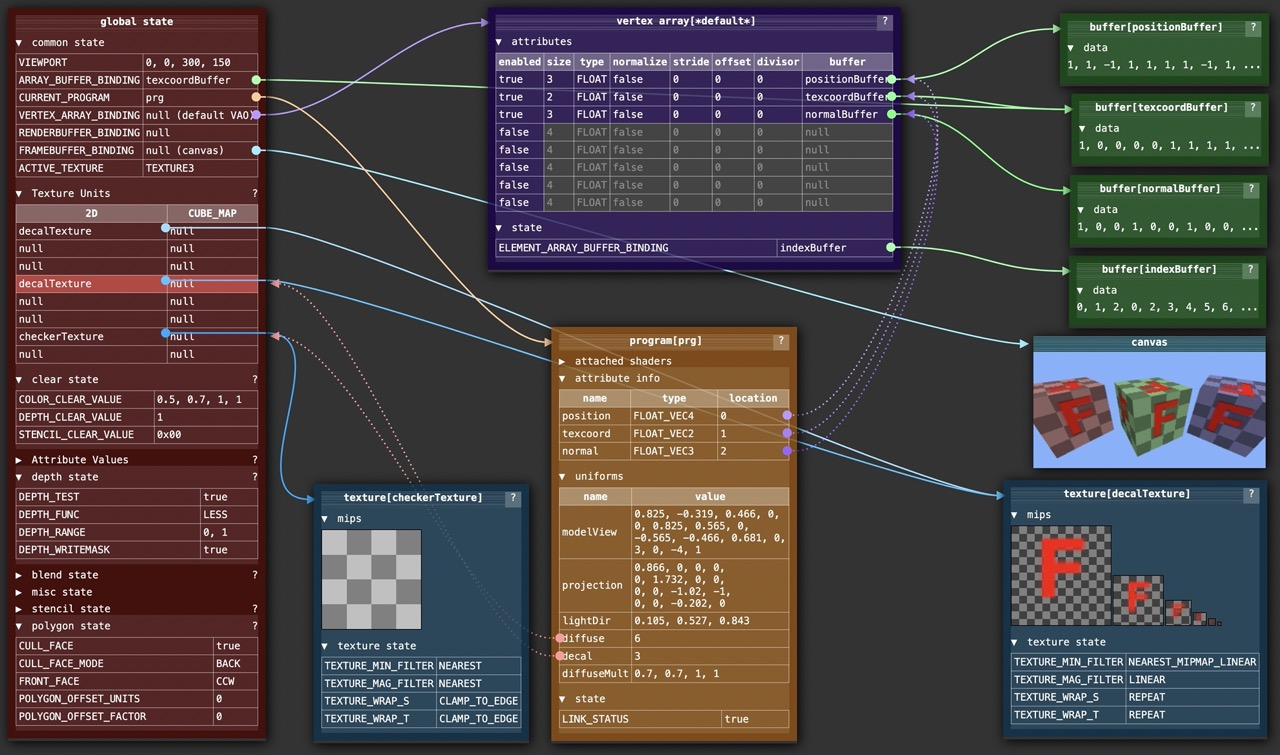
\includegraphics[width=\linewidth]{WebGLAndGlobalState.jpeg}
    \caption[De \textit{Global State} in \textit{WebGL}~\autocite{GFXFundamentals2024}]{Gebruik van een globale variable binnen WebGL~\autocite{GFXFundamentals2024}.}
    \label{fig:WebGL Global State}
\end{figure}

\textit{WebGL} gebruiken voor \textit{GPGPU} is echter een complexe implementatie die gebruik maakt van een \textit{global state} die volgens \textcite{Surma2022} al snel kan leiden tot een complexe code, en hierdoor ook tot fouten. Een schematische voorstelling van deze \textit{global state} wordt weergegeven in figuur \ref{fig:WebGL Global State}. De implementatie van \textit{GPGPU} werd door de introductie van \textit{Transform Feedback} in \textit{WebGL 2.0} toegankelijker. Dit is een simpelere methode om de data uit te lezen na een complexe berekening op de grafische kaart aan de hand van \textit{WebGL}. De data zit namelijk hierdoor in een eendimensionale reeks en is hierdoor makkelijker om verder mee te verwerken~\autocite{Tavares2021}. Maar deze nieuwere versie van \textit{WebGL} die \textit{Transform Feedback} beschikbaar stelt, werd pas in september 2021 ondersteund door \textit{Apple} op \textit{Safari}~\autocite{Surma2022}.

\bigbreak{}

\textit{WebGPU} vervangt dit \textit{global state} gedrag met \textit{pipelines} die niet aanpasbaar zijn eenmaal ze zijn aangemaakt~\autocite{Beaufort2023}. En omdat \textit{compute shaders} beschikbaar zijn is de \textit{Transform Feedback} oplossing is niet meer nodig bij \textit{WebGPU}. Het gebruiken van WebGL voor \textit{GPGPU} is niet enkel complex, het is ook inefficiënt. Data moet eerst als een \textit{texture} worden gecodeerd, daarna gedecodeerd in een \textit{shader}. Op dat moment moeten de eigenlijke berekeningen worden uitgevoerd. De resultaten van deze berekeningen moeten daarna opnieuw worden gecodeerd tot een \textit{texture}, alvorens er met de data kan worden verder gewerkt~\autocite{Surma2022}.

\bigbreak{}

Deze lange onnodige complexiteit komt verder uit het feit dat \textit{WebGL} werd ontworpen voor het visualiseren van grafische elementen en niet om algemene computationele taken uit te voeren zoals \textit{machine learning} of het mijnen van \textit{crypto currency}. Zoals eerder vermeld verbeterde de situatie wel met \textit{WebGL 2.0}, maar de ondersteuning hiervoor was beperkt en hierdoor kwam de proliferatie van lokale rekenkracht in de browser niet tot stand.

\break{}

\section{Introductie van WebGPU}
\label{sec:IntroWebGPU}

Omdat \textit{WebGPU} wordt gestandaardiseerd door het \textit{World Wide Web Consortium}, krijgt het ook de nodige ondersteuning om een potentiële standaard te worden zoals \textit{WebGL}. Een globaal initiatief kan er toe leiden dat deze technologie een revolutie betekent voor grafische weergave en lokale rekenkracht op het Web. In tegenstelling tot de beperkte ondersteuning waar \textit{WebGL 2.0} op kon rekenen, zitten bij \textit{WebGPU} wel alle browserfabrikanten mee in het ontwikkelingsproces~\autocite{Surma2022}.

\bigbreak{}

De werking van een GPU is heel complex. Hier wordt vaak te snel over gegaan. Er wordt door meerdere applicaties simultaan data naar het beeldscherm geprojecteerd waarbij de grafische kaart wordt opgedeeld. De veiligheidsimplicaties hiervan zijn niet te onderschatten, omdat deze applicaties elkaar niet mogen kunnen beïnvloeden of data van elkaar mogen uitlezen. Voor elke applicatie lijkt het dat deze over een monopolie beschikt van een grafische kaart. Uiteraard is dit niet het geval en wordt eigenlijk de rekenkracht verdeeld. Dit leidt ertoe dat de status van uitgevoerde taken moet worden bijgehouden omdat er altijd parallel wordt gewerkt. Programmeren voor \textit{General Purpose GPU} verloopt altijd op een \textit{multithreaded} asynchrone manier, waar rekening mee moet gehouden worden~\autocite{Surma2022}.

\bigbreak{}

Uiteraard zijn er al meerdere implementaties van \textit{machine learning} op het web, maar deze worden beschikbaar gesteld door servers en er wordt nog geen gebruik gemaakt van \textit{client-sided \textit{WebGPU} rendering}. \textcite{Fleetwood2023a} beweert dat het essentieel zal zijn dat modellen lokaal worden gedraaid om de echte \textit{real-time} te ondersteunen. Ook wanneer meerdere AI-modellen serieel worden gebruikt, om de functionaliteit van webapplicaties uit te breiden, verhoogt de vraag naar rekencapaciteit.

\bigbreak{}

Ook \textcite{Huyen2023} merkt in haar onderzoek op dat de kost van het draaien van AI-modellen in een productieomgeving enorm hoog kan oplopen. Hierdoor komt de rendabiliteit in gevaar. Dit is echter enkel het geval wanneer modellen suboptimaal worden ingezet zoals \textcite{Fleetwood2023a} opmerkt.

\begin{displayquote}[{\cite{Fleetwood2023a}}]
    "Offloading some parts of the call chain to finetuned local models could dramatically reduce costs while offering additional benefits such as privacy and personalization."
\end{displayquote}

\bigbreak{}

De \textit{WebGPU Shading Language} \(\textit{WGSL}\) \autocite{W3C2024}, is al opgemerkt als een moeilijke programmeertaal om mee te werken~\autocite{Madrigal2023, Ashton2020}.

Volgens \textcite{Fleetwood2023a} is dit echter niet het geval en hij vindt dat de syntax toegankelijk is omdat het veel invloeden heeft van \textit{Rust}, een populaire opkomende taal.

\bigbreak{}

\textit{WebGPU} laat toe dat er rekenkracht beschikbaar wordt gesteld aan de browser maar dit wil niet zeggen dat hiermee het probleem van de werking van complexe modellen lokaal in de browser is opgelost. Er is namelijk ook een geheugenlimiet omdat een model moet worden ingeladen. Hiervoor gaat de voorkeur naar het gebruik van het geheugen van de grafische kaart, indien deze te klein is geeft dit merkbare prestatiebeperkingen. Er kan hierdoor potentieel een \textit{bottleneck} ontstaan. Het efficiënt inladen en beschikbaar stellen van deze modellen is essentieel.

\section{WebGPU in vergelijking met WebGL}

Uit de ondervindingen van \textcite{Radin2021} blijkt dat \textit{WebGPU} tot drie maal sneller kan zijn dan WebGL in simpele matrix multiplicatie. Dit komt enerzijds omdat het proces om de berekeningen uit te voeren met \textit{WebGPU} een stuk eenvoudiger is, maar ook omdat \textit{WebGPU} \textit{compute shaders} ondersteunt in tegenstelling tot \textit{WebGL}. Om berekeningen uit te voeren met \textit{WebGL} is het namelijk vereist dat de data eerst wordt omgezet naar pixels zodat deze met een \textit{pixel shader} kunnen worden berekend zoals eerder vermeld in sectie \ref{sec:PowerOnWeb}. 

\bigbreak{}

Nog een nadeel van de afhankelijkheid op de \textit{pixel shader} van \textit{WebGL} is dat er gebruik moet gemaakt worden van het canvas object. \textcite{Radin2021} ondervond dat \textit{WebGL} matrix multiplicatie niet ondersteunt boven de 4096 x 4096, \textit{WebGPU} kon echter berekeningen uitvoeren tot matrices van 5000 x 5000. Het is ook belangrijk hierbij op te merken dat berekeningen uitgevoerd met \textit{WebGPU} asynchroon zijn wat eigen is aan grafische kaarten en \textit{GPGPU} zoals eerder vermeld in sectie \ref{sec:IntroWebGPU}. Dit feit valt ook uit te lezen op basis van de resultaten van \textcite{Radin2021} in figuur \ref{fig:Matrix Multiplication By Radin} waarbij duidelijk is dat bij de \textit{JavaScript} implementatie berekeningen relatief tot de \textit{GPU} implementaties initieel sneller beginnen. De begrenzingen van rekenkracht met \textit{JavaScript} op de processor worden echter wel snel duidelijk, hierbij kunnen matrices niet meer worden uitgevoerd wanneer deze te groot worden. Dit geldt ook voor de \textit{WebGL} implementatie maar dat is pas  bij grotere matrices.

\bigbreak{}

De \textit{GPU} implementaties van de test van \textcite{Radin2021} blijven met grotere matrices verder werken. De verschillen tussen \textit{WebGPU} en \textit{WebGL} manifesteren zich wel in het uiteenlopen van de uitvoeringstijd. Hierbij stijgt de benodigde tijd voor \textit{WebGL} sneller dan die van \textit{WebGPU} voor identieke matrices. Dit komt onder andere omdat er geen conversie moet worden uitgevoerd van en naar de \textit{GPU buffer} bij \textit{WebGPU}, wat wel het geval is bij \textit{WebGL} zoals eerder vermeld in sectie \ref{sec:PowerOnWeb}. 

\break{}

\begin{figure}
    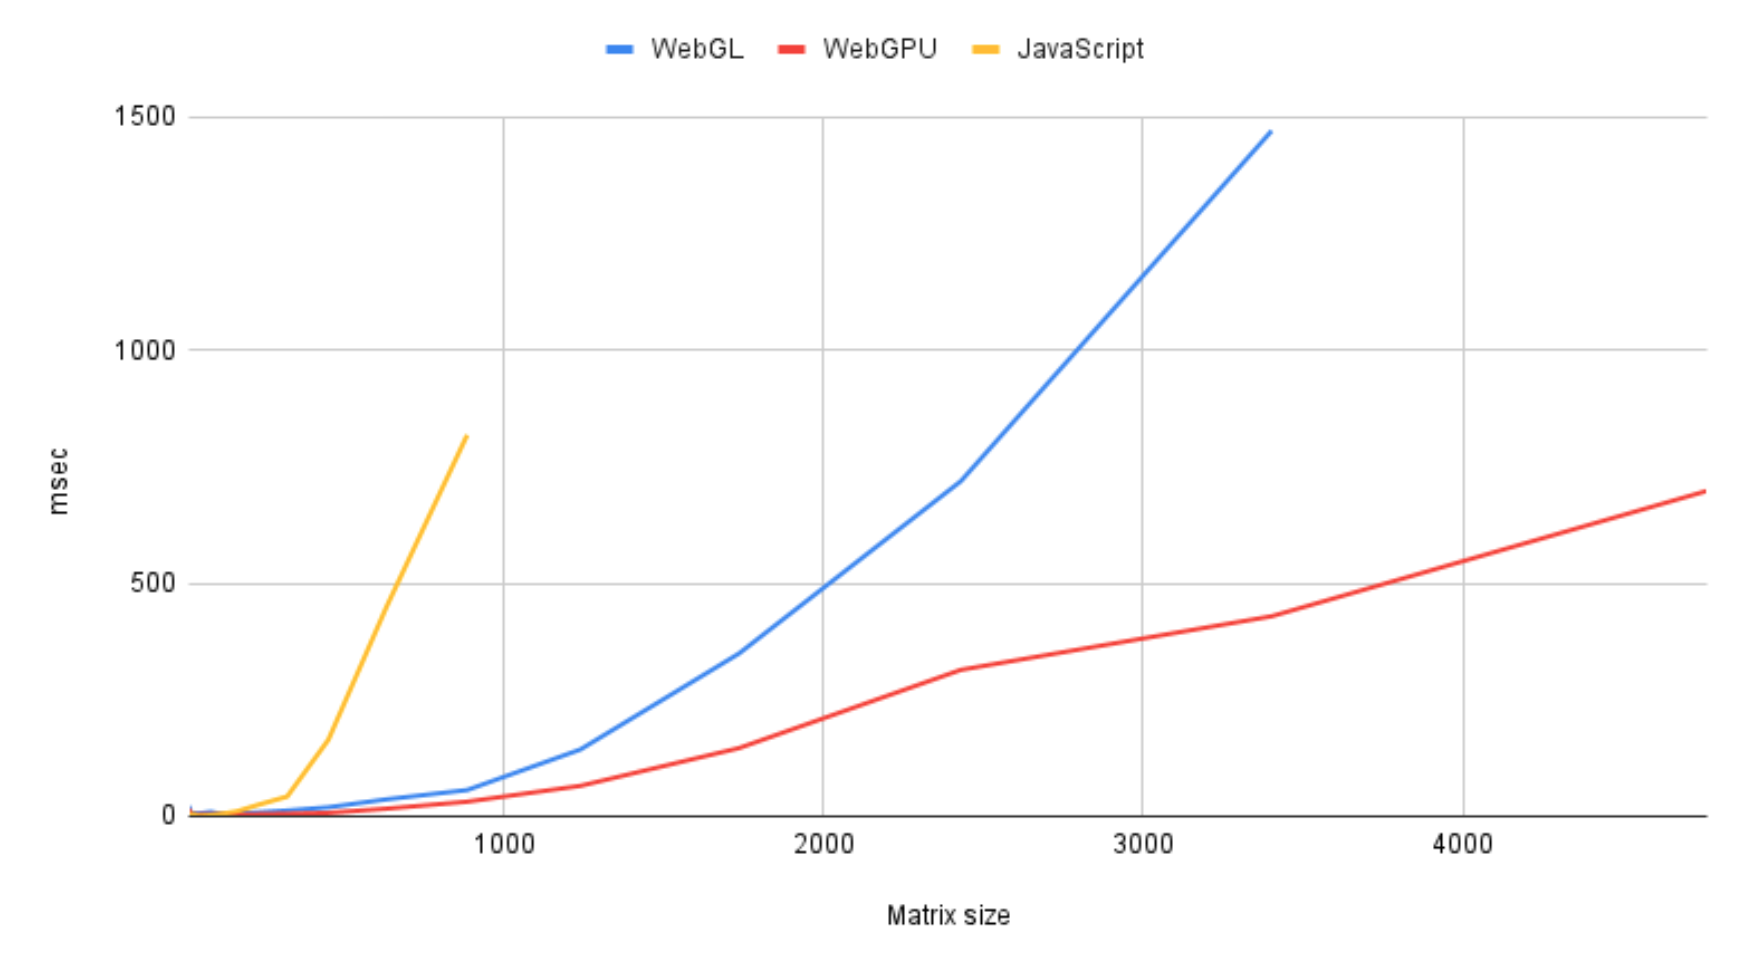
\includegraphics[width=\linewidth]{RadinMatrixMultiplicatie.png}
    \caption[Matrixvermenigvuldiging test~\autocite{Radin2021}]{Een test waarbij de prestaties van WebGPU, WebGL en \textit{JavaScript} werden vergeleken~\autocite{Radin2021}.}
    \label{fig:Matrix Multiplication By Radin}
\end{figure}

Het asynchrone gedrag en de efficiëntere implementatie van \textit{WebGPU} dragen toe aan het feit dat \textit{JavaScript} implementaties die gebruik maken van \textit{WebGPU} een lagere \textit{overhead} hebben. Dit betekent dat de achterliggende processor waarop \textit{JavaScript} code wordt uitgevoerd minder zwaar belast wordt. Door middel van zwaardere berekeningen uit te besteden aan de grafische kaart beschikbaar gesteld door API's zoals \textit{WebGL} en nu ook \textit{WebGPU}.

\begin{displayquote}[{\cite{Wallez2023}}]
    "As an example of the efficiency gains this can bring, an initial port of an image diffusion model in TensorFlow.js shows a 3x performance gain on a variety of hardware when moved from WebGL to WebGPU."
\end{displayquote}

De prestatie verbeteringen die \textcite{Wallez2023} bij het gebruik van \textit{TensorFlow.js} opmerkt worden niet enkel bevestigt wanneer er vergeleken wordt tussen \textit{WebGPU} en \textit{WebGL}. Ook in sectie \ref{sec:transformerbench} worden gelijkaardige resultaten behaald. De \textit{embedding} prestaties van zowel \textit{WebGPU} als \textit{Web Assembly} (\textit{WASM}), een compacte \textit{assembly-like binary} die prestaties op het web toelaat vergelijkbaar met \textit{native} talen zoals \textit{C/C++} en \textit{Rust} \autocite{Steiner2023}, werden hier met elkaar vergeleken.

\bigbreak{}

De ondervindingen van \textcite{Wallez2023} en \textcite{Radin2021} worden opnieuw bevestigd waarbij de \textit{embedding} prestaties, een process waarbij data in een vector databank wordt verwerkt zodat hierbij verbindingen kunnen worden gelegd \autocite{Cloudflare2024, Cloudflare2024a, Huyen2023}, ook hoger liggen wanneer \textit{WebGPU} wordt vergeleken met een processor implementatie zoals \textit{WASM} voor \textit{use cases} zoals het trainen van AI-modellen.

\break{}

\section{Het nut van lokale rekenkracht in de browser} 

\textcite{Fleetwood2022} merkt op dat er een paradigma verandering aankomt in hoe AI-modellen worden getraind. De huidige technologie werkt als volgt: informatie wordt door de gebruiker voorzien en opgestuurd naar een model dat beschikbaar is in de \textit{cloud} en dit model produceert een antwoord dat terug aan de gebruiker wordt voorgelegd.

\bigbreak{}

Dit paradigma is enigszins statisch, omdat het model dat draait in de \textit{cloud} niet veranderlijk is. \textcite{Fleetwood2022} gelooft dat een standaard met modellen die dynamisch opgebouwd worden, de toekomst is. Dit wil zeggen dat gewichten die worden toegepast op een AI-model gepersonaliseerd zijn voor de gebruiker. 

\bigbreak{}

Wanneer gewichten worden toegepast op AI-modellen kan het gedrag worden aangepast. Omdat AI-modellen worden opgebouwd met een enorme hoeveelheid data die niet altijd perfect is, kunnen er kleine aanpassingen worden gedaan door parameters te veranderen. Hierbij worden gewichten toegevoegd aan zaken die relevanter zijn. Dit gebeurd bij het training process wanneer een AI-model wordt geoptimaliseerd~\autocite{Hubbard2024}.

\begin{displayquote}[{\cite{Fleetwood2022}}]
    "It would be optimal if the subset of weights that get updated to learn about the user remained on their device."
\end{displayquote}

Het is duidelijk dat gepersonaliseerde AI-modellen die dynamisch worden opgebouwd een impact hebben op de privacy- en veiligheidsaspecten. Deze gevoelige informatie kan namelijk ook worden misbruikt wanneer deze in de foute handen valt. Het gebruik maken van AI-modellen die niet lokaal werken kunnen mogelijks lekken veroorzaken van geheime of gevoelige bedrijfsinformatie~\autocite{Wiggers2023, Sabin2023}. Het valt op te merken dat lokale beschikbaarheid van rekenkracht op het web door middel van \textit{WebGPU} een katalysator kan zijn voor een  revolutionaire verandering in privacy en veiligheid op het web.

\bigbreak{}

Wat \textcite{Fleetwood2022} ook opmerkt is dat er bij het draaien van  AI-technologieën vaak meerdere processen serieel werken. Juist omdat er verder wordt gewerkt op informatie die reeds werd gegenereerd, leent deze technologie zich voor een tussenoplossing. Deze zou toestaan een hybride \textit{cloud} te maken waarbij een deel van de computationele taken worden overgedragen aan de eindgebruiker.

\bigbreak{}

Er moet nog wel worden benadrukt dat het downloaden van AI-modellen een groot struikelblok voor de technologie kan vormen. Veel AI-modellen worden niet publiek gemaakt, hierbij kan geen gebruik worden gemaakt van een \textit{WebGPU} implementatie. AI-modellen die te groot zijn zorgen ervoor dat de eindgebruiker initieel moet wachten. Dit kan leiden tot een verminderde bruikbaarheid. Maar volgens \textcite{Fleetwood2022} zijn dit problemen die door middel van compressie en \textit{caching} grotendeels verholpen kunnen worden.

\break{}

\begin{figure}
    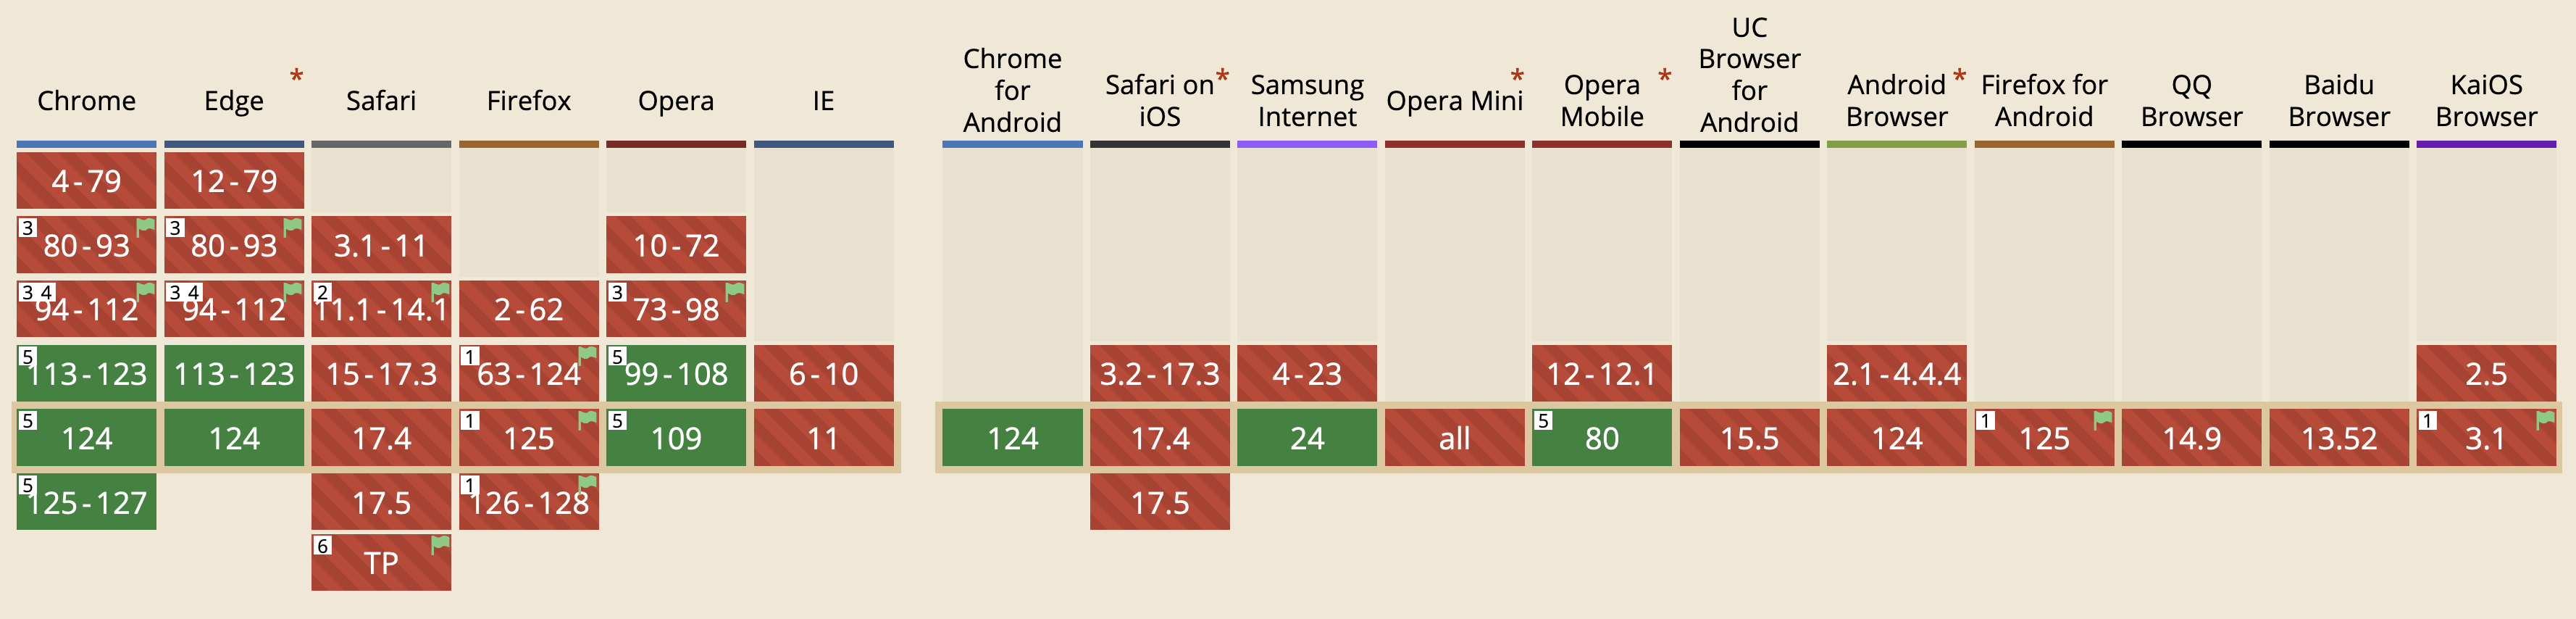
\includegraphics[width=\linewidth]{browsersupport.png}
    \caption[Ondersteuning voor \textit{WebGPU}~\autocite{Deveria2024}]{
        De \textit{Browser} ondersteuning voor \textit{WebGPU} te vinden op \href{https://caniuse.com/webgpu}{caniuse.com/webgpu}~\autocite{Deveria2024}.
    }
    \label{fig:Browser Support}
\end{figure}

\begin{figure}
    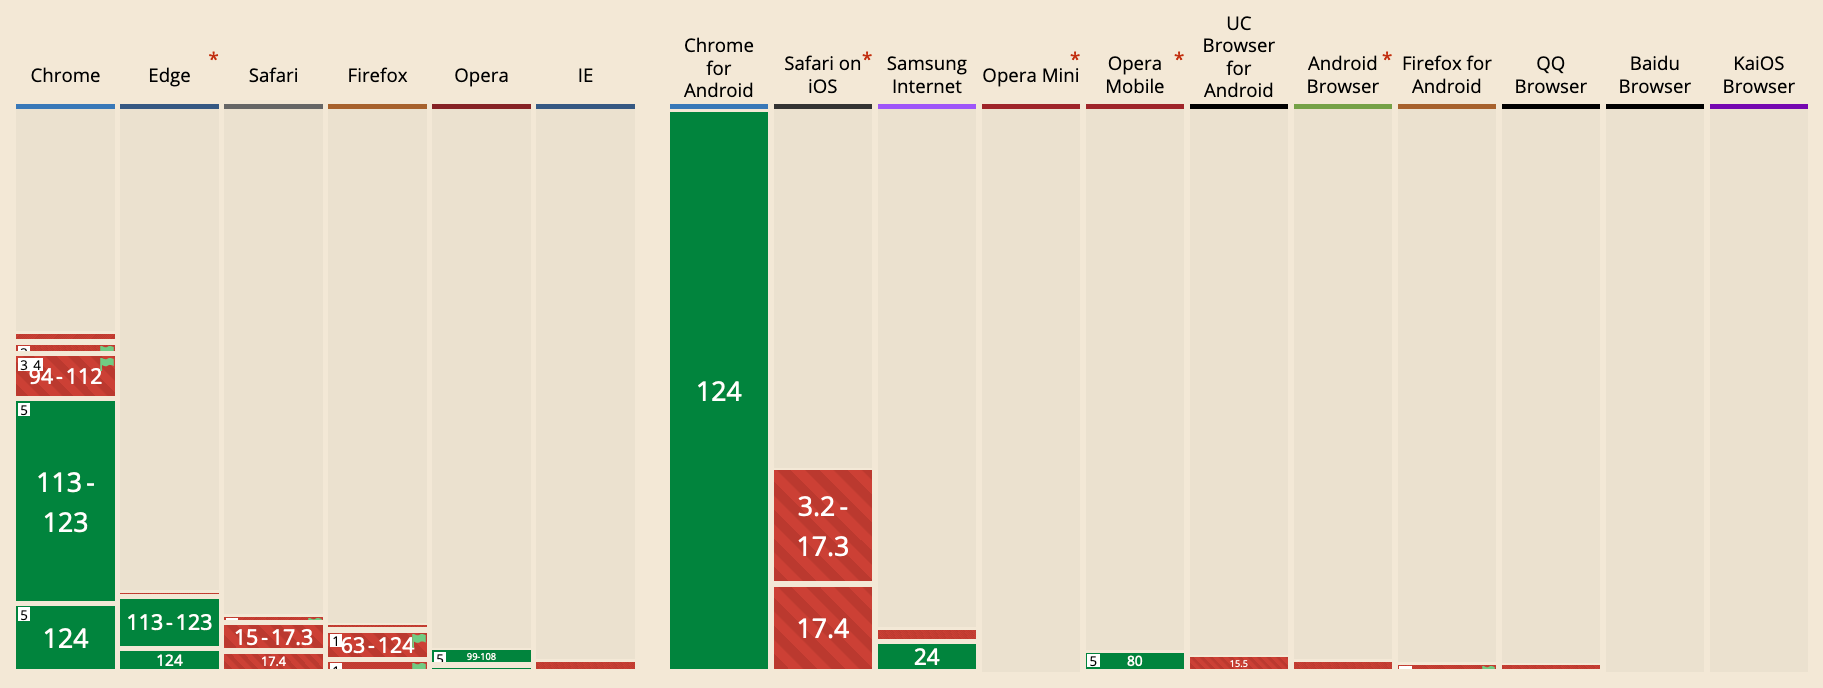
\includegraphics[width=\linewidth]{browsersupportuserrelative.png}
    \caption[Eindgebruikers met toegang tot \textit{WebGPU}~\autocite{Deveria2024}]{
        Ondersteuning voor \textit{WebGPU} te vinden op \href{https://caniuse.com/webgpu}{caniuse.com/webgpu} relatief tot gebruikers~\autocite{Deveria2024}.
    }
    \label{fig:Relative Browser Support}
\end{figure}

\section{WebGPU browser ondersteuning}

WebGPU wordt nog niet door alle browsers ondersteund. Het is belangrijk dat de \textit{early-adopter} gebruikers verifiëren dat hun browser compatibel is. Dit kan makkelijk worden uitgezocht aan de hand van \href{https://caniuse.com/webgpu}{caniuse.com}. Omdat \textit{WebGPU} een relatief nieuwe technologie is, wordt deze soms enkel in testversies ondersteund. Zie \textit{Firefox} met groene vlagjes op afbeelding \ref{fig:Browser Support}. Merkwaardig is ook dat \textit{Chrome} volledige ondersteuning biedt op de desktop- en mobiele markt ~\autocite{Deveria2024}.

\bigbreak{}
\newdate{date}{06}{05}{2024}
\date{\displaydate{date}}

Afbeelding \ref{fig:Browser Support} toont de ondersteuning voor \textit{WebGPU} binnen verschillende \textit{browsers}; deze worden horizontaal weergegeven. Ook verschillende versies van specifieke \textit{browsers} worden telkens verticaal opgelijst. Omdat er veel versies rood worden aangeduid zou kunnen worden afgeleid dat ondersteuning voor \textit{WebGPU} nog niet is doorgebroken, dit is echter niet het geval. Afbeelding \ref{fig:Relative Browser Support} toont namelijk een correcter beeld. Hierbij is de grafiek omgevormd relatief tot de verdeling van het aantal gebruikers. Op  \displaydate{date} heeft 70,51\% van de totale browser gebruikers toegang tot \textit{WebGPU}, volgens statistische informatie beschikbaar gesteld door \textcite{Deveria2024}.

\section{Realistisch scenario's simuleren met WebGPU}

\begin{figure}
    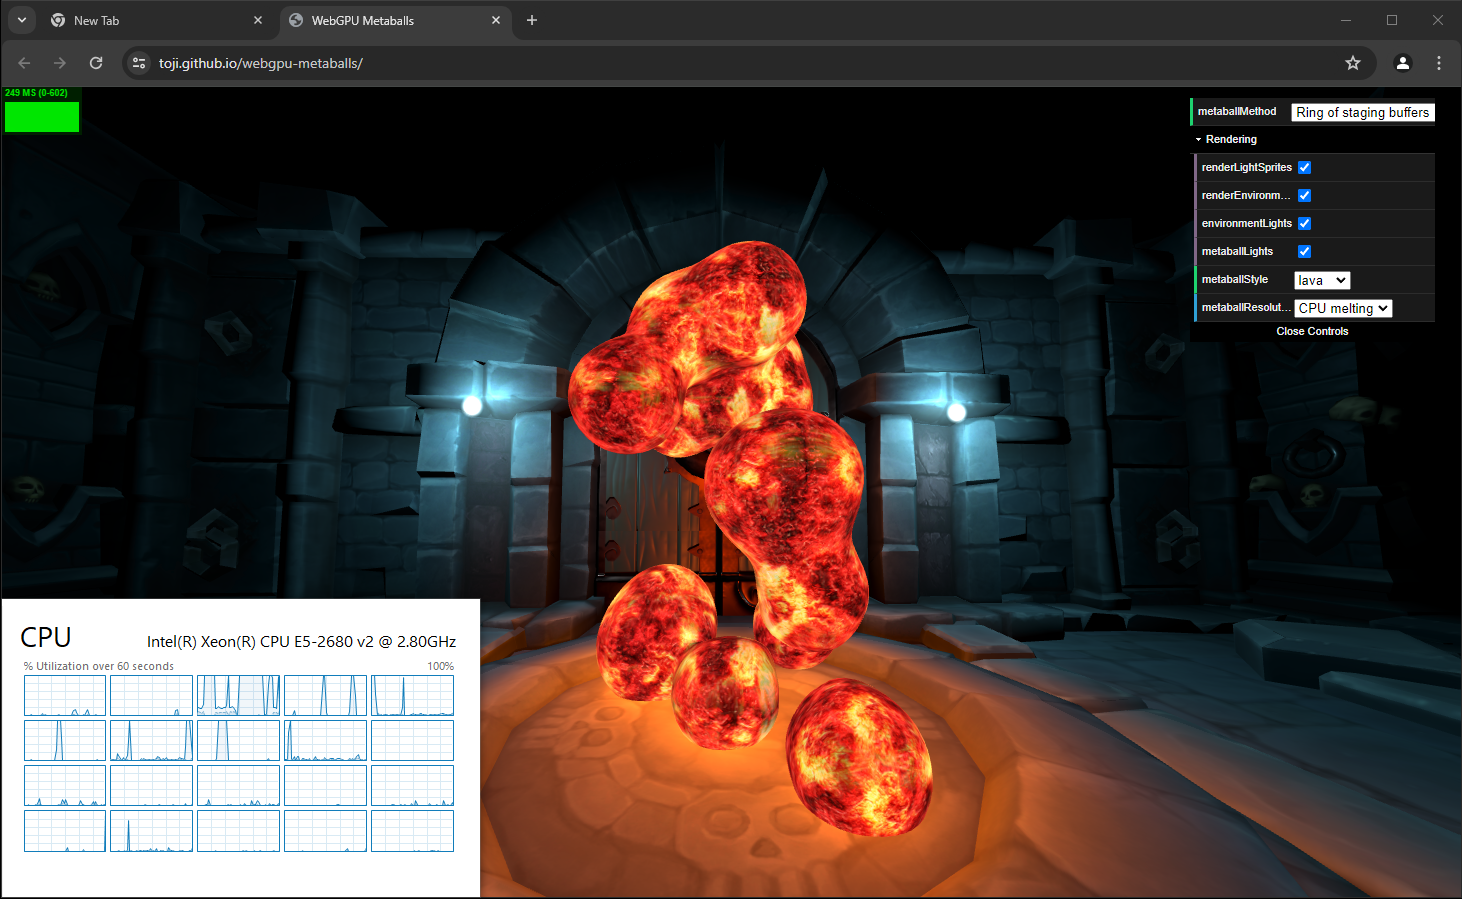
\includegraphics[width=\linewidth]{MetaBallsSimulationJS.png}
    \caption[\textit{JavaScript} implementatie van vloeistof simulatie~\autocite{Jones2024}]{
        \textit{JavaScript} implementatie van vloeistof simulatie waarbij het CPU gebruik hoog ligt en enkel kan worden uitgevoerd op een kern. \textit{JavaScript} vertraging wordt linksboven aangeduid in milliseconden~\autocite{Jones2024}.
    }
    \label{fig:MetaBallsSimulationJS}
\end{figure}

\begin{figure}
    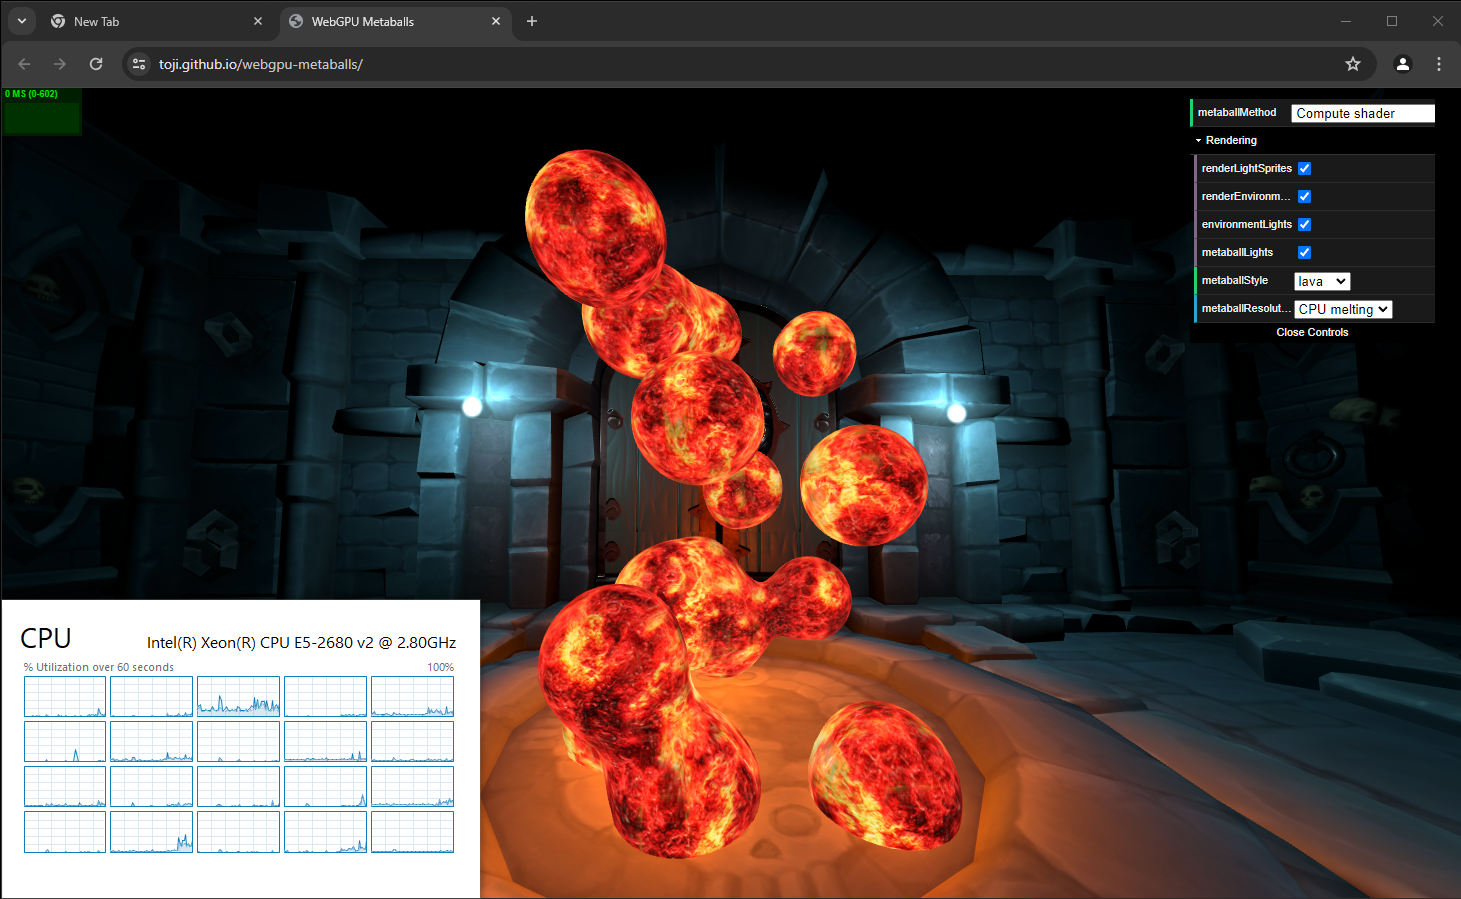
\includegraphics[width=\linewidth]{MetaBallsSimulationWebGPU.png}
    \caption[\textit{WebGPU} implementatie van vloeistof simulatie~\autocite{Jones2024}]{
        \textit{WebGPU} implementatie van vloeistof simulatie waarbij de benodigde berekeningen worden uitgevoerd op de grafische kaart. \textit{JavaScript} vertraging wordt linksboven aangeduid in milliseconden~\autocite{Jones2024}.
    }
    \label{fig:MetaBallsSimulationWebGPU}
\end{figure}

\textit{WebGPU} biedt niet enkel verbeteringen op vlak van \textit{GPGPU}. Deze technologie kan ook worden ingezet voor het produceren van individuele \textit{frames} wanneer simulaties worden uitgevoerd. Hierbij moeten zaken uit de fysica worden gesimuleerd. Implementaties aan de hand van \textit{WebGPU} laten dit opnieuw op een efficiëntere manier toe. Wanneer berekeningen voorheen werden uitgevoerd in \textit{JavaScript}, kunnen deze nu worden overgedragen aan de grafische kaart~\autocite{Wallez2023}.

\bigbreak{}

Dit kan worden gedemonstreerd aan de hand van het voorbeeld van \textcite{Jones2023}. Op afbeelding \ref{fig:MetaBallsSimulationJS} is een \textit{JavaScript} implementatie zichtbaar van het \textit{marching cubes algorithm}. Hierbij wordt een vloeistof gesimuleerd. Het interageren tussen de oppervlaktes van de bellen moet worden weergegeven. De berekeningen die hiervoor vereist zijn worden in dit voorbeeld uitgevoerd met \textit{JavaScript}. De processor wordt hierbij dus zwaar belast en dit valt zeker te merken want de simulatie begint sterk te haperen. 

\bigbreak{}

Parallel rekenkracht met \textit{Javascript} is beperkt. Bij deze simulatie wordt zelfs maar één kern gebruikt. Dit is zichtbaar in de taakbeheer grafiek links beneden op afbeelding \ref{fig:MetaBallsSimulationJS} waarbij de processor belasting per kern wordt weergegeven. De simulatie loopt hierbij een sterke vertraging op van 250 milliseconden per \textit{frame}.

\bigbreak{}

Wanneer de instelling in dit voorbeeld echter wordt aangepast naar \textit{compute shaders} verdwijnt de \textit{JavaScript} vertraging zo goed als volledig. Dit kan worden uitgelezen op afbeelding \ref{fig:MetaBallsSimulationWebGPU}, waarbij het processor verbruik sterk is gedaald. Ook de JavaScript vertraging is gezakt naar nul milliseconden. Hierdoor kan de simulatie stabiel op 60 \textit{frames} per seconden worden uitgevoerd. En de processor wordt niet meer zwaar belast waardoor andere zaken op de webpagina \textit{responsive} blijven.

\bigbreak{}

Het is belangrijk te vermelden dat \textit{WebGPU} niet enkel vernieuwingen brengt in de vorm van algemene rekenkracht, maar ook de grafische prestaties verschillen tussen \textit{WebGL 2.0} en \textit{WebGPU}~\autocite{Wallez2023}. 

\bigbreak{}
Grafische weergave op het web werd sinds 2011 afgehandeld door \textit{WebGL}. Deze technologie was echter verouderd en werd vervangen met \textit{WebGL 2.0} in 2017~\autocite{Surma2022}. Sinds \textit{WebGL 2.0} zijn er nieuwere grafische technologieën op de markt zoals \textit{ray tracing}, waarbij individuele fotonen worden getraceerd om extreem realistische belichting te simuleren. Deze nieuwe technologieën werden niet verwerkt in \textit{WebGL} maar worden wel verwacht in \textit{WebGPU}~\autocite{Surma2022}. \textit{WebGPU} laat dus uiteraard niet enkel verbeteringen toe op vlak van \textit{GPGPU} en simulaties van realistische scenario's, maar ook voor normaal gebruik van de grafische kaart binnen de browseromgeving.
%%=============================================================================
%% Methodologie
%%=============================================================================

\chapter{\IfLanguageName{dutch}{Methodologie}{Methodology}}%
\label{ch:methodologie}

%% TODO: In dit hoofstuk geef je een korte toelichting over hoe je te werk bent
%% gegaan. Verdeel je onderzoek in grote fasen, en licht in elke fase toe wat
%% de doelstelling was, welke deliverables daar uit gekomen zijn, en welke
%% onderzoeksmethoden je daarbij toegepast hebt. Verantwoord waarom je
%% op deze manier te werk gegaan bent.
%% 
%% Voorbeelden van zulke fasen zijn: literatuurstudie, opstellen van een
%% requirements-analyse, opstellen long-list (bij vergelijkende studie),
%% selectie van geschikte tools (bij vergelijkende studie, "short-list"),
%% opzetten testopstelling/PoC, uitvoeren testen en verzamelen
%% van resultaten, analyse van resultaten, ...
%%
%% !!!!! LET OP !!!!!
%%
%% Het is uitdrukkelijk NIET de bedoeling dat je het grootste deel van de corpus
%% van je bachelorproef in dit hoofstuk verwerkt! Dit hoofdstuk is eerder een
%% kort overzicht van je plan van aanpak.
%%
%% Maak voor elke fase (behalve het literatuuronderzoek) een NIEUW HOOFDSTUK aan
%% en geef het een gepaste titel.

\section{literatuurstudie}

De wereld van WebGPU is heel nieuw en klein, het is echter belangrijk op te merken dat heel grote bedrijven deze technologie ondersteunen en er actief aan mee werken. 

\section{Introductie tot WebGPU en shaders}

De eerste stap nadat het theoretische onderzoek werd afgerond was het uitwerken van een simpele demonstratie. Uit de literatuurstudie bleek dat het uitwerken van complexe zaken een te grote stap was. Een implementatie van \textit{Conway's Game of Life} was echter wel geschikt als introductie.

\section{Requirement analyse}

Het toegangelijk maken van kunstmatige intelligentie via het web is een grote uitdaging die tot nu toe gepaard gaat met enorme 

\section{long list van technologieen}

Verzamelen van reeds bestaande technologieen en beschrijven waartoe deze in staat zijn.

\section{Short list van technologieen}

\section{Proof of Concept}

Een belangrijk element van

\section{Conclusie}




% Voeg hier je eigen hoofdstukken toe die de ``corpus'' van je bachelorproef
% vormen. De structuur en titels hangen af van je eigen onderzoek. Je kan bv.
% elke fase in je onderzoek in een apart hoofdstuk bespreken.

\chapter{Meetresultaten}%
\label{ch:benchmarks}

De performantie van \textit{WebGPU} in vergelijking met andere technologieën kan sterk verschillen. Om een beeld te vormen over de capaciteiten die \textit{WebGPU} brengt, worden in dit hoofdstuk enkele testen uitgevoerd. Hierdoor kan er vergeleken worden hoe de prestaties van \textit{WebGPU} al dan niet overeenstemmen met traditionele \textit{GPGPU} technologieën zoals \textit{CUDA}, of normale rekenkracht beschikbaar gesteld door een \textit{Central Processing Unit} (\textit{CPU}).

\section{Transformer prestaties van WASM en WebGPU}

Een andere opkomende technologie is \textit{web assembly} (\textit{WASM}). \textit{WASM} is een zeer compact \textit{assembly-like binary} die performantie toelaat vergelijkbaar met \textit{native} talen zoals \textit{C/C++} en \textit{Rust}~\autocite{Steiner2023}.

\begin{displayquote}[{\cite{Chen2020}}]
    "We introduced support for WASM and WebGPU backends to the Apache TVM deep learning compiler. Our initial experiments shows that TVM's WebGPU backend can get close to native GPU performance when deploying models in the browser."
\end{displayquote}

Deze \textit{low-level} programmeertalen laten net zoals \textit{WGSL} voor \textit{WebGPU} toe dat rekenkundige taken optimaal worden uitgevoerd. Dit komt omdat de code specifiek wordt geschreven op een manier die rekening houdt met hoe de onderliggende hardware functioneert~\autocite{Knight2020}.

\begin{figure}
    \centering
    \pgfplotsset{width=15cm,compat=1.9}

% We will externalize the figures
% \tikzexternalize
\pgfplotsset{
  log ticks with fixed point,
}
\begin{tikzpicture}
    \begin{semilogxaxis}[
        title={Transformer benchmark fp32 WASM versus WebGPU},
        xlabel={Batch size},
        ylabel={Uitvoeringstijd in ms},
        xmin=1, xmax=64,
        ymin=0, ymax=70000,
        xtick={1,2,4,8,16,32, 64},
        ytick={1,10000,20000,30000,400000,50000,60000, 70000},
        legend pos=north west,
        ymajorgrids=true,
        grid style=dashed,
        scatter/classes={
            a={mark=square*,red},
            b={mark=triangle*,orange},
            c={mark=o,draw=blue},
            d={mark=square,green}
        },
        yticklabel style={
            /pgf/number format/fixed,
        },
        scaled y ticks=false
    ]
    
        \addplot[
            color=red,
            mark=square*
            ]
            coordinates {
                (1, 946.14)(2, 1923.12)(4, 3816.90)(8, 7653.00)(16, 15494.62)(32, 30901.40)(64, 61788.00)
            };
            \addlegendentry{WASM (fp32) Intel Xeon E5-2680 V2}
            
        \addplot[
            color=orange,
            mark=triangle*
            ]
            coordinates {
                (1, 747.10)(2, 1499.98)(4, 3014.38)(8, 5956.38)(16, 11807.70)(32, 24121.56)(64, 47769.14)
            };
            \addlegendentry{WASM (fp32) Intel Core i9-9980HK}
        \addplot[
            color=blue,
            mark=o
            ]
            coordinates {
                (1, 193.66)(2, 365.90)(4, 703.24)(8, 1393.12)(16, 2752.66)(32, 5510.74)(64, 10966.04)
            };
            \addlegendentry{WebGPU (fp32) Intel UHD Graphics 630}

        \addplot[
            color=green,
            mark=square
            ]
            coordinates {
                (1, 28.02)(2, 58.28)(4, 77.74)(8, 116.40)(16, 226.00)(32, 463.16)(64, 739.16)
            };
            \addlegendentry{WebGPU (fp32) Nvidia Geforce GTX 1080 Ti}
        \addplot [
            scatter,only marks,
            scatter src=explicit symbolic,
        ] table [x=x,y=y,meta=label] {plotdata/HuggingFaceWasmVSWebGPU.dat};

    \end{semilogxaxis}
\end{tikzpicture}
    \label{sec:transformerbench}
\end{figure}

\subsection{Uitvoeren van de test}

De performantie van verschillende testopstellingen werd opgemeten aan de hand van de \textit{webgpu-embedding-benchmark} van \textcite{Lochner2024}. Hierbij blijkt \textit{WebGPU} consistent sneller dan \textit{WASM} voor zowel sterke als zwakke grafische kaarten. In deze test werd de uitvoeringstijd gemeten van \textit{BERT-based embedding} modellen met zowel \textit{WebGPU} als \textit{WASM}, en dit telkens voor een toenemende \textit{batch size}.

\bigbreak{}

Voor een \textit{batch-size} van 64 doet de \textit{Xeon E5-2680 V2} gemiddeld 60 seconden over de \textit{transformer} test. Wanneer deze tijd als basis wordt genomen is de \textit{Intel Core i9-9980HK 10} seconden sneller.

\subsection{Vergelijken van resultaten}

Een veel gebruikte standaard om rekenkracht van computer onderdelen te vergelijken is door het aantal berekeningen van comma getallen per seconden op te meten. Deze berekening wordt uit gedrukt in \emph{floating point operations per second} (\textit{FLOPS}) en laat dus toe om algemene rekenkracht van verschillende componenten te vergelijken. 

\bigbreak{}

Zowel theoretische waarden als meetresultaten werden telkens vergeleken met de \textit{base line} gebaseerd op de performantie van de \textit{Xeon E5-2680 v2}. Bij het uitvoeren van deze testen werd de sequentie lengte steeds ingesteld op 512. Deze lengte beschrijft het aantal \textit{tokens} die samen worden gegroepeerd door de \textit{transformer}. Ook werden alle testen uitgevoerd met \emph{Chrome versie 124}.

\break{}

\begin{table}[t]
    \begin{tabular}{ |p{5.5cm}|p{2.5cm}|p{2.5cm}|p{3.5cm}|  }
        \hline
        \multicolumn{4}{|c|}{Vergelijken van theoretische \textit{Floating Point} prestaties met meetresultaten} \\
        \hline
        Component& Theoretisch GFLOPS & Theoretisch vergelijking & Resultaten transformertest\\
        \hline
            Xeon E5-2680 V2             & 224,0     & 100\%  & 100\%       \\
            Intel Core i9-9980HK        & 307,2     & 137\%  & 129\%    \\
            Intel UHD Graphics 630      & 403,2     & 180\%  & 560\%    \\
            Nvidia GeForce GTX 1080 Ti  & 11.340,0  & 5063\% & 7170\%   \\
        \hline
    \end{tabular}
    \caption[\textit{Floating point} performantie \textit{CPU's} en \textit{GPU's} \autocite{Intel2024, Intel2024a, TechPowerUp2017, TechPowerUp2017a}]{Theoretische floating point performantie \autocite{Intel2024, Intel2024a, TechPowerUp2017, TechPowerUp2017a}}
    \label{tab:TheoreticalVersusMeasuredPerf}
\end{table}

In tabel \ref{tab:TheoreticalVersusMeasuredPerf} werd de \textit{Xeon E5-2680 v2} als basis gebruikt om de andere componenten te vergelijken. Omdat de \textit{Intel Core i9-9980HK} een nieuwere processor is, is deze gemiddeld voor alle \textit{batch} groottes 29\% sneller. Ook werd de theoretische snelheid van deze componenten opgenomen in deze table zodat er kan vergeleken worden of de meetresultaten overeen komt met wat theoretisch verwacht wordt van de individuele componenten. 

\bigbreak{}

Voor beide processoren werd de Intel specificatie gebruikt om de theoretische \textit{GFLOPS} te bepalen~\autocite{Intel2024, Intel2024a}. De \textit{GFLOPS} voor de grafische kaarten werd gebaseerd op informatie die beschikbaar werd gesteld door \textcite{TechPowerUp2017, TechPowerUp2017a}.

\subsection{Conclusie}

Uit de grafiek en de tabel valt af te leiden dat voor deze test \textit{WebGPU} een geschikte technologie is voor het trainen van AI-modellen op de browser. De test duidt ook aan dat het inzetten van de grafische kaart voor deze \textit{embedding} berekeningen een geschiktere component is dan een processor implementatie.

\bigbreak{}

Ook valt af te leiden uit de resultaten van de \textit{Embedding Benchmark} van \textcite{Lochner2024} dat \textit{WebGPU} beter presteert dan verwacht uit de theoretische snelheden. Dit ligt aan de implementatie van de test. Net zoals \textit{WebGPU} is \textit{WebAssembly} een nieuwe technologie. Beide technologieën zijn nog in ontwikkeling en kunnen verder verbetert worden. Dit blijkt ook uit de testen die in sectie \ref{sec:whispertest} werden uitgevoerd. De resultaten van de \textit{WASM} testen liggen dichter bij de theoretische verwachtingen. Dit wijst erop dat de \textit{WASM} implementaties onderpresteren maar wel correct schalen bij krachtigere processoren. Hierdoor lijken de \textit{WebGPU} resultaten een stuk beter dan wat theoretisch verwacht werd.

\break{}

\section{Whisper implementaties met CPU, \textit{CUDA} en WebGPU}%
\label{sec:whispertest}

Het Whisper AI-model van \textcite{OpenAI2023} wordt online gepubliceerd met verschillende parameter groottes. Een model neemt steeds meer geheugen in naarmate het aantal parameters stijgt en er geen optimalisaties worden uitgevoerd. Hierdoor kan met deze modellen goed getest worden omdat de prestaties beïnvloed worden door het aantal parameters. Er geldt wel een begrenzing voor apparaten met beperkt geheugen. Niet alle apparaten hebben namelijk evenveel beschikbaar geheugen, en kunnen dus niet alle Whisper modellen uitvoeren. 

\bigbreak{}

Grafische kaarten laten niet enkel hoge parallellisatie toe, maar hebben in het algemeen ook een veel hogere geheugen bandbreedte dan het RAM-geheugen van een processor zie tabel \ref{tab:RAMSpeeds}. Deze bandbreedte speelt ook een rol bij het uitvoeren van inferentie, en heeft dus effect op hoe snel het \textit{Whisper} model een audio fragment kan interpreteren.

\bigbreak{}

\textit{Whisper} kan als module in \textit{Python} worden geïmporteerd. Door een testscript te schrijven kunnen verschillende model-groottes worden ingeladen. Dit script kan worden teruggevonden in de bijlage sectie \ref{sec:whispertestcode}. Ook laat de \textit{Whisper} module in \textit{Python} toe om alsnog de CPU te gebruiken. Wanneer \textit{torch} wordt geïnstalleerd voor \textit{Python} kan deze ook worden ingesteld om gebruik te maken van \textit{CUDA}. Hierna kan de \textit{Whisper} module het \textit{CUDA} apparaat gebruiken op \textit{Python}. \textit{WebGPU} kon getest worden met Whisper omwille van de implementaties van \textcite{Fleetwood2024, Fleetwood2023b}.

\bigbreak{}

De modellen van OpenAI met verschillende parameter groottes zijn beschikbaar op \href{https://github.com/openai/whisper}{GitHub.com/OpenAI/Whisper}. De modellen die zijn opgelijst in tabel \ref{tab:OpenAIWhisperModels}, werden allemaal getest met \textit{CUDA} en processor implementaties in \textit{Python}. De base, small en large modellen werden getest met WebGPU.

\begin{table}[b]
    \begin{tabular}{ |p{1.6cm}|p{2.5cm}|p{2.7cm}|p{2.7cm}|p{1.9cm}|p{1.8cm}|  }
        \hline
        \multicolumn{6}{|c|}{Beschikbare modellen en talen Whisper} \\
        \hline
            Grootte& Parameters & English-only model & Multilingual model & Vereiste VRAM & Relatieve snelheid\\
        \hline
            tiny&       39 M    &tiny.en    & tiny& ~1 GB& ~32x     \\
            base &      74 M	&base.en    & base & ~1 GB & ~16x   \\
            small &     244 M	&small.en   & small & ~2 GB & ~6x   \\
            medium &    769 M	&medium.en  & medium & ~5 GB & ~2x  \\
            large &     1550 M	&N/A        & large & ~10 GB& 	1x  \\
        \hline
    \end{tabular}
    \caption{Whisper modellen beschikbaar gesteld door \textcite{OpenAI2023}.}
    \label{tab:OpenAIWhisperModels}
\end{table}

\break{}

\subsection{Uitvoeren van Python test script}

Omdat Whisper zoveel verschillende modelgroottes beschikbaar stelt maakt dit het AI-model zeer geschikt om te testen met \textit{WebGPU}, maar ook met \textit{CUDA} en normale processor implementaties. Door verschillende grafische kaarten en processoren te testen kon hierdoor een beeld gegeven worden wat de verwacht prestaties zijn die \textit{WebGPU} kan bieden in vergelijking met normale processoren of geavanceerdere \textit{CUDA} implementaties. De invloed van de toenemende parameter grootte op de uitvoeringstijd kan hierdoor ook duidelijk worden gerepresenteerd.

\bigbreak{}

Om testresultaten op een consistente manier te verzamelen werd een \textit{Python} script geschreven. Dit script werd dan op verschillende apparaten uitgevoerd om op deze manier betrouwbare data te verzamelen. Er werd telkens gebruik gemaakt van \textit{Python} versie 3.11, in combinatie met \textit{torch} en \textit{torchaudio} versie 2.0.0+cu117 en \textit{torchvision} versie 0.15.0+cu117.

\bigbreak{}

Om de prestaties van \textit{WebGPU} te onderzoeken werd de implementatie van \textcite{Fleetwood2024} gebruikt. Deze geeft namelijk telkens de inferentie tijd weer, die nodig was voor het uitvoeren. Deze data werd manueel verzameld.

\bigbreak{}

\subsection{Installatie afhankelijkheden}

Om \textit{Whisper} operationeel te krijgen op een \textit{Windows 10} installatie zijn er verschillende afhankelijkheden die moeten worden geïnstalleerd. Dit betreft \textit{Python 3.9.9}, \textit{PyTorch 1.10.1} en de \textit{CUDA toolkit}. Het is ook belangrijk op te merken dat Torch moet worden gecompileerd met \textit{CUDA} functionaliteit, indien dit niet wordt gedaan, kan enkel door middel van de processor de \textit{Whisper} modellen worden uitgevoerd.

\subsection{Opzetten van de test}

Zowel \textit{Windows 10} als \textit{Ubuntu server 22.04} werden getest met versies van \textit{Whisper} ondersteund door \textit{CUDA} en \textit{CPU}. Maar om de performantie van \textit{WebGPU} te kunnen vergelijken met \textit{CUDA} werd enkel op \textit{Windows 10} getest met een \textit{Nvidia GeForce GTX 1080 Ti} grafische kaart. Hierdoor kon consistente data verzameld worden.

\break{}

% PS > pip3 uninstall torch torchvision==0.15.0 torchaudio==2.0.0
% PS > pip3 cache purge
% PS > pip3 install torch torchvision==0.15.0 torchaudio==2.0.0 --index-url https://download.pytorch.org/whl/cu117

% import torch
% torch.cuda.is_available()
% # returns False
% torch.zeros(1).cuda()
% # throws AssertionError: Torch not compiled with CUDA enabled

% \begin{lstlisting}[language=Python]
% import torch
% torch.cuda.is_available()
% # returns True
% torch.zeros(1).cuda()
% # returns tensor([0.], device='cuda:0')
% \end{lstlisting}
\begin{figure}
    \centering
    \pgfplotsset{width=15cm,compat=1.9}

\pgfplotsset{
  log ticks with fixed point,
}

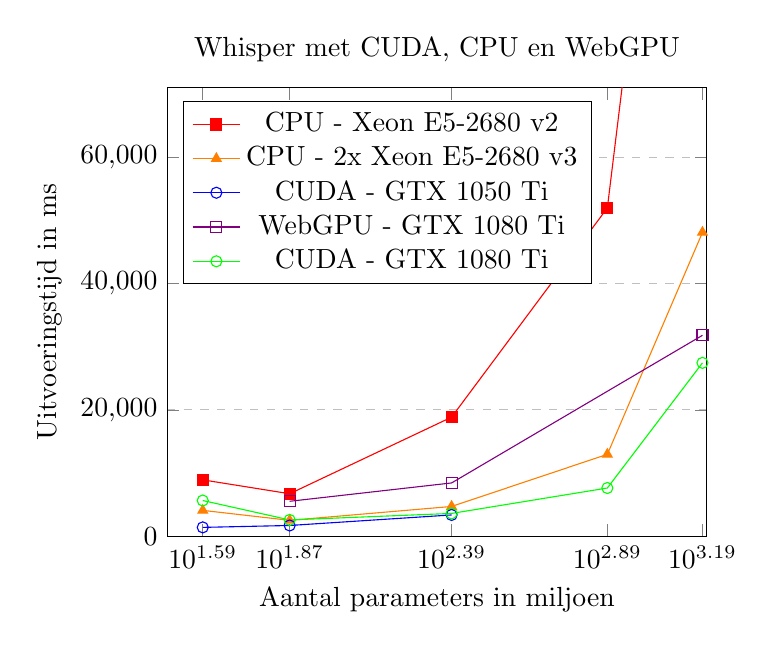
\begin{tikzpicture}
    \begin{semilogxaxis}[
        title={Whisper met CUDA, CPU en WebGPU},
        xlabel={Aantal parameters in miljoen},
        ylabel={Uitvoeringstijd in ms},
        xmin=30, xmax=1600,
        ymin=0, ymax=71000,
        xtick={39, 74, 244, 769, 1550},
        legend pos=north west,
        ymajorgrids=true,
        grid style=dashed,
        yticklabel style={
            /pgf/number format/fixed,
        },
        scaled y ticks=false
    ]
    \addplot[
            color=red,
            mark=square*
        ]
        coordinates {(39,8919)(74,6721)(244,18849)(769,51980)(1550,175378)};
        \addlegendentry{CPU - Xeon E5-2680 v2}

    \addplot[
        color=orange,
        mark=triangle*
        ]
        coordinates {(39,4088)(74,2508)(244,4706)(769,12963)(1550,48107)};
        \addlegendentry{CPU - 2x Xeon E5-2680 v3}

    \addplot[
            color=blue,
            mark=o
        ]
        coordinates {(39,1393)(74,1694)(244,3362)};
        \addlegendentry{CUDA - GTX 1050 Ti}
    
    \addplot[
            color=violet,
            mark=square
        ]
        coordinates {(74,5526)(244,8431)(1550,31814)};
        \addlegendentry{WebGPU - GTX 1080 Ti}

    \addplot[
            color=green,
            mark=o
        ]
        coordinates {(39,5647)(74,2574)(244,3602)(769,7629)(1550,27448)};
        \addlegendentry{CUDA - GTX 1080 Ti}
    \end{semilogxaxis}
\end{tikzpicture}
\end{figure}

% pip3 install torch torchvision==0.15.0 torchaudio==2.0.0 --index-url https://download.pytorch.org/whl/cu117
% pip3 install torch torchvision==0.15.0 torchaudio==2.0.0 --index-url https://download.pytorch.org/whl/cpu
% pip3 uninstall torch torchvision==0.15.0 torchaudio==2.0.0
% pip3 cache purge

\subsection{Resultaten van de Whisper test}

Uit de resultaten kan worden afgeleid dat zelfs krachtige processoren zoals de Xeon E5-2680 v2 en v3 al snel niet op kunnen tegen de parallelle rekenkracht van grafische kaarten. De experimentele \textit{WebGPU} implementatie van \textcite{Fleetwood2024} kan niet evenaren aan de \textit{CUDA} implementatie deze verschillen gemiddeld 53,4\%, 57,2\% en 13,7\% bij de \textit{base}, \textit{small} en \textit{large} implementaties van \textit{Whisper} respectievelijk. Relatief gezien ten opzichte van de processor prestaties van de \textit{Xeon E5-2680 v2} is dit geen groot verschil, omdat deze processor prestaties naarmate dat het \textit{Whisper} model wordt uitgevoerd met toenemende parameter grootte niet goed schaalt.

\bigbreak{}

Het is wel belangrijk te vermelden dat bij de \textit{large} implementatie van \textit{Whisper} het \textit{VRAM} geheugen gebruik van het model substantieel lager was in \textit{WebGPU} dan in de \textit{CUDA} implementatie en dat hierdoor het model mogelijks een andere kwantisatie wordt toegepast. Dit kan leiden tot een verlaagd \textit{VRAM} gebruik.

\bigbreak{}

Initieel presteren de twee \textit{Xeon E5-2680 v3} processoren beter dan de \textit{WebGPU} implementatie. Maar naarmate het model in parameter grootte toeneemt wordt duidelijk dat de uitvoeringstijd sterk begint te stijgen. De verhoogde parallelle rekenkracht van de grafische kaarten zijn hiertegen beter opgewassen. Ook speelt de verhoogde \textit{VRAM} bandbreedte hier een rol. Het verschil in RAM bandbreedte van de processoren en grafische kaarten kan worden vergeleken in table \ref{tab:RAMSpeeds}. 

\bigbreak{}

Omwille van het beperkte geheugen waarover de \textit{GTX 1050 Ti} beschikt (4GB) kon deze enkel worden getest tot en met het kleine \textit{Whisper} model (244 miljoen parameters). Dit is een belangrijke beperking om in acht te houden bij gebruiken grafische kaarten voor de uitvoering van AI-modellen. Wanneer \textit{WebGPU} of \textit{CUDA} technologie wordt gebruikt om AI-modellen uit te voeren moet er rekening worden gehouden hoeveel beschikbaar werkgeheugen er is. Wanneer deze grens wordt bereikt, wordt vaak het gedeelde geheugen gebruikt. Hierdoor wordt de bandbreedte sterk beperkt omdat er een constante uitwisseling moet plaats vinden tussen het geheugen van de grafische kaart en het geheugen van de processor.

\subsection{Conclusie}

De \textit{Xeon} processoren die gebruikt werden voor deze test zijn niet representatief voor een eindgebruiker. Deze processor opstelling vertegenwoordigd een traditionele server implementatie. Het is belangrijk om op te merken dat processoren van de eindgebruiker meestal niet kunnen evenaren aan deze processor prestaties. Deze Xeon processoren werden getest om een vergelijking te maken met hoe het \textit{Whisper} model kan worden geïmplementeerd aan de server kant, en welke prestaties hierbij kunnen worden verwacht. Er kan namelijk niet realistisch worden verwacht van eindgebruikers om complexe software zoals CUDA te installeren zodat het Whisper model kan worden gebruikt. Daarom zou deze implementatie moeten worden uitgevoerd op een server waarop een eindgebruiker dan toegang tot heeft.

\bigbreak{}

Performante grafische kaarten daarentegen zijn wel beschikbaar voor de eindgebruiker omwille van de proliferatie van videogames. Een implementatie van het \textit{Whisper} model op de browser kan zeker voordelen geven wanneer deze gebruik kan maakt van lokale componenten. Ook laat het lokaal verwerken van audio een verhoogde privacy toe voor de eindgebruiker. En wanneer een webapplicatie die het \textit{Whisper} model lokaal implementeert wordt omgevormd tot een \textit{PWA} kan deze zelf offline gebruikt worden.

\begin{table}[b]
    \begin{tabular}{ |p{6cm}|p{3cm}|p{3cm}|p{3cm}|  }
        \hline
        \multicolumn{4}{|c|}{\textit{Random Access Memory} snelheden} \\
        \hline
        Component& DDR generatie & Klokfrequentie & Bandbreedte \\
        \hline
            Xeon E5-2680 V2             & DDR 3     & 1866 MHz  & 59.7 GB/s \\
            2x Xeon E5-2680 V3          & DDR 4 ECC & 2133 MHz  & 136 GB/s  \\
            Nvidia GeForce GTX 1050 Ti  & GDDR 5    & 7008 MHz  & 112.1 GB/s\\
            Nvidia GeForce GTX 1080 Ti  & GDDR 5X   & 11000 MHz & 484.4 GB/s\\
        \hline
    \end{tabular}
    \caption[Verschillen in RAM snelheden voor \textit{CPU's} en \textit{GPU's}~\autocite{Intel2013,Intel2014,TechPowerUp2016, TechPowerUp2017}]{\textit{Random Access Memory} snelheden van \textit{CPU's} volgens \textcite{Intel2013,Intel2014} en \textit{GPU's} volgens \textcite{TechPowerUp2016, TechPowerUp2017}}
    \label{tab:RAMSpeeds}
\end{table}

%\input{...}
%...

%%=============================================================================
%% Conclusie
%%=============================================================================

\chapter{Conclusie}%
\label{ch:conclusie}

% TODO: Trek een duidelijke conclusie, in de vorm van een antwoord op de
% onderzoeksvra(a)g(en). Wat was jouw bijdrage aan het onderzoeksdomein en
% hoe biedt dit meerwaarde aan het vakgebied/doelgroep? 
% Reflecteer kritisch over het resultaat. In Engelse teksten wordt deze sectie
% ``Discussion'' genoemd. Had je deze uitkomst verwacht? Zijn er zaken die nog
% niet duidelijk zijn?
% Heeft het onderzoek geleid tot nieuwe vragen die uitnodigen tot verder 
%onderzoek?

% Is \textit{WebGPU} een geschikte technologie om de rekenkracht die vereist is bij het operationeel inzetten van kunstmatige intelligentie op grote schaal over te dragen aan de eindgebruiker. Staat deze overdracht een verbetering toe voor de gebruikservaring en vraag naar privacy?

% Om antwoord te geven op de onderzoeksvraag die voor dit onderzoek werd gesteld; is \textit{WebGPU} een geschikte technologie overeenstemt met het potentiële evenaren of overstemmen van de huidige technologie die word onderzocht. Hierbij spelen gebruiksvriendelijkheid en de kans op meer privacy ook een rol.

% \bigbreak{}

\iffalse
TODO Samen hang moet worden verbetert, alle zaken die hier besproken zijn geweest moeten zeker aan bod zijn gekomen in het onderzoek! Al dan niet verder in detail bespreken.
\fi

Het beschikbaar stellen van AI-modellen in webapplicaties en software blijkt een bewezen interessante investering te zijn voor bedrijven die de functionaliteit van webapplicaties sterk willen uitbreiden. Hierbij wordt de eindgebruiker mogelijks gedwongen gebruik te maken van de externe diensten waardoor de kosten sterk kunnen oplopen. Ook kan de bescherming van de privacy van de eindgebruiker niet altijd gegarandeerd worden. Deze twee minpunten zijn te vermijden bij het gebruik van \textit{WebGPU}.

\bigbreak{}

Door verschillende testen uit te voeren, werd de rekencapaciteit van \textit{WebGPU} onderzocht. Uit deze resultaten werd geconcludeerd dat \textit{WebGPU}, zoals verwacht, een hoge rekencapaciteit kan ontgrendelen, die voorheen enkel beschikbaar was door \textit{lower-level APIs} te gebruiken zoals \textit{Metal}, \textit{Direct3D}, \textit{Vulcan} of \textit{OpenGL}.

\bigbreak{}

Sterker nog, \textit{WebGPU} toont niet alleen de capaciteit om  AI-modellen voor normaal gebruik te kunnen ondersteunen, maar ook te kunnen trainen. Het feit dat de benodigde \textit{hardware} afhankelijk wordt van de eindgebruiker moet natuurlijk in acht worden gehouden, maar omdat voor 70\% van de internet gebruikers \textit{WebGPU} beschikbaar is, laat \textit{WebGPU} toe deze hardware ook verder te kunnen inzetten binnen een browser omgeving. Dit wijst erop dat \textit{WebGPU} in staat is zijn om de proliferatie van lokale inferentie mogelijk te maken, waardoor de minpunten van externe diensten geëlimineerd wordt.

\bigbreak{}

Uiteraard is \textit{WebGPU} niet de enige technologie die hand in hand gaat met de opkomst van kunstmatige intelligentie. Ook computer fabrikanten zoals Microsoft zijn actief bezig met het ondersteunen van lokale inferentie~\autocite{Mehdi2024}. Veel technologieën worden ontwikkeld met lokale uitvoering van AI-modellen als basis. Er kan dus worden vastgesteld dat hoe dan ook lokale inferentie op de apparatuur van de eindgebruiker een technologie is die zich nu persisteert in de markt.

\bigbreak{}

Gedurende dit onderzoek werd vast gesteld dat de nieuwe implementaties van \textit{WebGPU} technologie nog steeds volop ontwikkeld worden. Hierbij werd vooral opgemerkt dat de combinatie van \textit{WebGPU} met kunstmatige intelligentie verder begon uitgewerkt te worden door verschillende ontwikkelaars. Dit leidde ertoe dat gedurende het uitwerken van dit onderzoek meerdere projecten met \textit{WebGPU} implementaties beschikbaar kwamen op \textit{GitHub} en \textit{Hugginface}. Veel van deze projecten zijn echter nog in experimentele fase maar kunnen toch al indrukwekkende resultaten behalen. Hiermee bewijzen deze technische implementaties dat \textit{WebGPU} een geschikte technologie is voor lokale inferentie of het web wanneer deze verder doorgroeit en ontwikkelt wordt. 

\bigbreak{}

Door deze conclusie te combineren met de eerder besproken toegankelijkheid van \textit{WebGPU} kan een krachtige synergie aangetoond worden die de eindgebruiker in staat zal stellen om applicaties op een gebruiksvriendelijke manier te installeren en te gebruiken. En dit zonder afhankelijk te moeten zijn van complexe achterliggende technologieën of externe diensten. Hierdoor wordt een implementatie van \textit{WebGPU} ontzettend aantrekkelijk voor kleinschalige softwareoplossingen die, in tegenstelling tot de voormalige grafische geaccelereerde software, zeer eenvoudig te onderhouden zijn.

\bigbreak{}

Niet enkel stelt \textit{WebGPU} de gebruiker in staat om deel te nemen aan de kunstmatige intelligentie \textit{gold rush}, het laat ook toe om dit op een privacybewuste manier te doen. Dit komt omdat er minimale datauitwisseling vereist is met externe diensten. Voor de toekomstige privacybewuste gebruiker kan \textit{WebGPU} technologie zeer waardevol worden. Hiervoor moet echter wel verder onderzocht worden wat de impact is van \textit{WebGPU} gebruikers op zaken zoals \textit{digital fingerprinting}. Ook moeten de cybersecurity aspecten van \textit{WebGPU} verder worden onderzocht. De technologie zou gevoelig kunnen zijn voor \textit{side channel attacks}~\autocite{Giner2024}.

\bigbreak{}

Naast het beschikbaar maken van lokale inferentie belooft \textit{WebGPU} nog veel andere innovaties voor de \textit{browsers}. Het is echter belangrijk dat het doelpubliek van webapplicaties wordt onderzocht, en dat hierbij wordt gekeken op welke achterliggende technologie deze software wordt uitgevoerd. Dit heeft namelijk een grote impact op welke AI-modellen kunnen worden gebruikt en hoe groot deze mogen zijn. Dit was namelijk ook merkbaar bij het uitvoeren van de \textit{web-llm} implementatie in het prototype. Er moet op basis van technologische capaciteiten van de apparaten van de eindgebruiker worden aanbevolen welk AI-model geschikte prestaties kan voorzien. De uitdaging voor \textit{browserfabrikanten} en web\-on\-twi\-kke\-laars zal zijn om van deze technologie optimaal gebruik te maken en hierdoor de \textit{WebGPU} (r)evolutie, ontwikkeling en implementatie voort te zetten.

%---------- Bijlagen -----------------------------------------------------------

\appendix

\chapter{Onderzoeksvoorstel}

Het onderwerp van deze bachelorproef is gebaseerd op een onderzoeksvoorstel dat vooraf werd beoordeeld door de promotor. Dat voorstel is opgenomen in deze bijlage.

%% TODO: 
\section*{Samenvatting}
% Kopieer en plak hier de samenvatting (abstract) van je onderzoeksvoorstel.

% Verwijzing naar het bestand met de inhoud van het onderzoeksvoorstel

% \begin{abstract}
In dit onderzoek wordt de integratie van kunstmatige intelligentie (AI) in \textit{Progressive Web Apps} (PWAs) door middel van WebGPU onderzocht. Deze integratie valt binnen het domein \textit{web development} en heeft tot doel het lokaal uitvoeren van AI-modellen te verkennen door gebruik te maken van WebGPU.\@ Door AI-modellen rechtstreeks in de browser te laten draaien wordt het installatieproces vereenvoudigd. Hierbij ligt de focus op de implementatie van AI-modellen, zoals onder andere het Whisper-model. Er wordt ook specifiek aandacht besteed aan potentiële voordelen op het gebied van prestaties en gebruikerservaring. Verwachte resultaten omvatten een vergelijkende analyse van de prestaties van WebGPU met bestaande renderer technologieën, zoals WebGL en CUDA. Dit onderzoek draagt bij aan de wetenschappelijke kennis over de synergie tussen AI, webtechnologieën en grafische rendering, met implicaties voor ontwikkelaars en professionals die betrokken zijn bij de integratie van AI in webomgevingen.
% \end{abstract}

%---------- Inleiding ---------------------------------------------------------

\section{Introductie}%
\label{sec:introductie}

% Waarover zal je bachelorproef gaan? Introduceer het thema en zorg dat volgende zaken zeker duidelijk aanwezig zijn:

% \begin{itemize}
%   \item kaderen thema
%   \item de doelgroep
%   \item de probleemstelling en (centrale) onderzoeksvraag
%   \item de onderzoeksdoelstelling
% \end{itemize}

% Denk er aan: een typische bachelorproef is \textit{toegepast onderzoek}, wat betekent dat je start vanuit een concrete probleemsituatie in bedrijfscontext, een \textbf{casus}. Het is belangrijk om je onderwerp goed af te bakenen: je gaat voor die \textit{ene specifieke probleemsituatie} op zoek naar een goede oplossing, op basis van de huidige kennis in het vakgebied.

% De doelgroep moet ook concreet en duidelijk zijn, dus geen algemene of vaag gedefinieerde groepen zoals \emph{bedrijven}, \emph{developers}, \emph{Vlamingen}, enz. Je richt je in elk geval op it-professionals, een bachelorproef is geen populariserende tekst. Eén specifiek bedrijf (die te maken hebben met een concrete probleemsituatie) is dus beter dan \emph{bedrijven} in het algemeen.

% Formuleer duidelijk de onderzoeksvraag! De begeleiders lezen nog steeds te veel voorstellen waarin we geen onderzoeksvraag terugvinden.

% Schrijf ook iets over de doelstelling. Wat zie je als het concrete eindresultaat van je onderzoek, naast de uitgeschreven scriptie? Is het een proof-of-concept, een rapport met aanbevelingen, \ldots Met welk eindresultaat kan je je bachelorproef als een succes beschouwen?

Dit onderzoek verkent de grenzen van webtechnologieën door zich te richten op de integratie van opensource kunstmatige intelligentie modellen met WebGPU. Hierbij wordt er ook onderzocht tot hoever deze kunnen worden ingebouwd in Progressive Web Apps (PWA's). 

\bigbreak{}
De snelle evolutie van webtechnologieën bieden nieuwe mogelijkheden voor het uitvoeren van complexe taken rechtstreeks in de browser. In het specifieke domein van AI en opensource-modellen presenteert dit onderzoek een innovatieve benadering waarbij WebGPU wordt ingezet voor de lokale uitvoering van AI-modellen.

\bigbreak{}
WebGPU laat toe; net zoals zijn voorganger WebGL, om grafische berekeningen uit te voeren op de GPU van de client. Dit biedt een alternatief voor de traditionele CPU-gebaseerde berekeningen, die vaak minder efficiënt zijn. WebGPU is een nieuwe standaard die momenteel in ontwikkeling is. Het is een low-level API die toegang geeft tot de GPU van de client.

\bigbreak{}
Naast verschuiving van rekenkracht van servers naar de client-side wat zorgt voor een enrome simplificatie op vlak van technologisch vereisten aan de serverkant. Richt dit onderzoek zich tevens ook op de gebruiksvriendelijkheid van AI-modellen binnen PWAs. Hierbij wordt onderzocht om het installatieproces van deze modellen te stroomlijnen en toegankelijk te maken voor een breder publiek. Omwille van de opkomst van WebGPU en de groeiende populariteit van PWAs, is dit onderzoek van groot belang voor de webgemeenschap.

\bigbreak{}
Dit onderzoek biedt waardevolle inzichten en relevante bevindingen voor ontwikkelaars binnen de domein mobiele en enterprise web development. Maar ook voor professionals en experts die betrokken zijn bij de integratie van kunstmatige intelligentie in webtoepassingen en de optimalisatie van grafische renderertechnologieën.

\newpage

%---------- Stand van zaken ---------------------------------------------------
\section{Stand van zaken}%
\label{sec:stand van zaken}

% Hier beschrijf je de \emph{state-of-the-art} rondom je gekozen onderzoeksdomein, d.w.z.\ een inleidende, doorlopende tekst over het onderzoeksdomein van je bachelorproef. Je steunt daarbij heel sterk op de professionele \emph{vakliteratuur}, en niet zozeer op populariserende teksten voor een breed publiek. Wat is de huidige stand van zaken in dit domein, en wat zijn nog eventuele open vragen (die misschien de aanleiding waren tot je onderzoeksvraag!)?

% Je mag de titel van deze sectie ook aanpassen (literatuurstudie, stand van zaken, enz.). Zijn er al gelijkaardige onderzoeken gevoerd? Wat concluderen ze? Wat is het verschil met jouw onderzoek?

% Verwijs bij elke introductie van een term of bewering over het domein naar de vakliteratuur, bijvoorbeeld~\autocite{Hykes2013}! Denk zeker goed na welke werken je refereert en waarom.

% Draag zorg voor correcte literatuurverwijzingen! Een bronvermelding hoort thuis \emph{binnen} de zin waar je je op die bron baseert, dus niet er buiten! Maak meteen een verwijzing als je gebruik maakt van een bron. Doe dit dus \emph{niet} aan het einde van een lange paragraaf. Baseer nooit teveel aansluitende tekst op eenzelfde bron.

% Als je informatie over bronnen verzamelt in JabRef, zorg er dan voor dat alle nodige info aanwezig is om de bron terug te vinden (zoals uitvoerig besproken in de lessen Research Methods).

% Voor literatuurverwijzingen zijn er twee belangrijke commando's:
% \autocite{KEY} => (Auteur, jaartal) Gebruik dit als de naam van de auteur
%   geen onderdeel is van de zin.
% \textcite{KEY} => Auteur (jaartal)  Gebruik dit als de auteursnaam wel een
%   functie heeft in de zin (bv. ``Uit onderzoek door Doll & Hill (1954) bleek
%   ...'')

% Je mag deze sectie nog verder onderverdelen in subsecties als dit de structuur van de tekst kan verduidelijken.

\subsection{Opkomst WebGPU}
In de dynamische wereld van webontwikkeling betreedt WebGPU als een relatief nieuwe speler het toneel, en het zal een golf van innovatie met zich mee brengen. Deze opkomende technologie, gericht op het verbeteren van de grafische prestaties binnen webomgevingen, staat nog in de beginfase van zijn ontwikkeling. Het besef van de nieuwheid van WebGPU onderstreept de noodzaak van grondig onderzoek om de volledige reikwijdte van zijn mogelijkheden te begrijpen en te benutten. 

\subsection{Kunstmatige Intelligentie}
De opkomst van kunstmatige intelligentie (AI) als een essentieel element binnen webtoepassingen voegt een extra dimensie toe aan de urgentie van onderzoek naar WebGPU.\@ In een tijdperk waarin AI-gebaseerde functies de norm worden, is het van cruciaal belang om te begrijpen hoe WebGPU deze evolutie kan ondersteunen en versterken. Het belang van deze synergie tussen WebGPU en AI versterkt de roep om diepgaand onderzoek, aangezien de webgemeenschap zich voorbereidt op een nieuwe fase van technologische vooruitgang.\autocite{Gu2023}

\subsection{Progressive Web Apps}
De integratie van opensource kunstmatige intelligentie modellen met WebGPU binnen Progressive Web Apps (PWAs), wordt de aanzienlijke waarde van PWAs als een moderne paradigmaverschuiving binnen webapplicaties benadrukt. 
\bigbreak{}
De PWAs, zoals gepresenteerd door \textcite{Shumylo2023}, zijn zorgvuldig vormgegeven om een ervaring te bieden die vergelijkbaar is met native apps, gebruikmakend van geavanceerde webtechnologieën zoals Service Workers, Web App Manifest, en Push Notifications.

\bigbreak{}
In tegenstelling tot traditionele webapplicaties vertoont het PWA-concept een reeks significante voordelen, waaronder versnelde laadtijden, robuuste offline-ondersteuning, een ervaring die parallel loopt aan native apps, grensoverschrijdende compatibiliteit, en moeiteloze ontdekbaarheid. Deze eigenschappen maken PWAs bijzonder geschikt als omgeving voor de uitvoering van complexe AI-taken aan de client-zijde, met de ondersteuning van WebGPU.\@

\bigbreak{}
Dit onderzoek richt zich op een grondige verkenning van de mogelijkheden om opensource AI-modellen te integreren in deze voor\-uit\-stre\-ven\-de webtoepassingen, 
met als doel de algehele gebruikerservaring te versterken en innovatieve inzichten te verschaffen binnen het domein van Mobile en Enterprise Development.

\subsection{WebGPU versus WebGL}

Het bestaande onderzoek naar de prestaties van WebGPU ten opzichte van WebGL, met inbegrip van evaluaties binnen de Godot-game-engine, bevestigt inderdaad de verbeterde prestaties van WebGPU volgens \textcite{Fransson2023}. Deze bevindingen benadrukken de substantiële vooruitgang die WebGPU biedt ten opzichte van bestaande renderertechnologieën zoals WebGL. De positieve resultaten in termen van prestatieverbeteringen onderstrepen het potentieel van WebGPU om een impactvolle rol te spelen in de optimalisatie van grafische weergave op het web.

\bigbreak{}
In hetzelfde licht staat de nieuwste versie van WebGL, die steunt op OpenGL ES 3.0, voor beperkingen met betrekking tot ray tracing-functies. Deze beperkingen onderstrepen het groeiende belang van opkomende technologieën zoals Web\-GPU. Deze renderbenaderingen kan worden mogelijk gemaakt door Compute shaders; die nu beschikbaar zijn in WebGPU volgens \textcite{Beaufort2023}.

\bigbreak{}
In tegenstelling tot de beperkingen van WebGL streeft WebGPU naar vernieuwing en verbetering van grafische mogelijkheden op het web, waaronder mogelijkheden die cruciaal zijn voor ray tracing. WebGPU belichaamt zo een veelbelovend alternatief, dat zich positioneert als een krachtige speler in de evolutie van grafische rendering op het web.

\subsection{JavaScript en WebGPU}

Workloads die eerder alleen in JavaScript konden worden uitgevoerd, kunnen nu naar de GPU worden verplaatst. Ook is WebGPU waardevol voor het versnellen van machine learning-taken op grafische kaarten. \autocite{Wallez2023}.

\bigbreak{}
Voorheen gebruikten ontwikkelaars WebGL's rendering API voor niet\-ren\-de\-ring operaties, zoals machine learning-be\-re\-ke\-ning\-en. Deze aanpak resulteerde echter in inefficiënties, zoals redundante geheugenladingen en suboptimale prestaties. WebGPU adresseert deze problemen met zijn belangrijkste nieuwe functie: compute shaders. Deze shaders bieden een flexibeler programmeermodel dat profiteert van de massaal parallelle aard van de GPU zonder beperkt te worden door de strikte structuur van renderoperaties.  Dit verbetert de efficiëntie aanzienlijk en optimaliseert de prestaties ten  opzichte van eerdere methoden met WebGL.

\newpage


%---------- Methodologie ------------------------------------------------------
\section{Methodologie}%
\label{sec:methodologie}

% Hier beschrijf je hoe je van plan bent het onderzoek te voeren. Welke onderzoekstechniek ga je toepassen om elk van je onderzoeksvragen te beantwoorden? Gebruik je hiervoor literatuurstudie, interviews met belanghebbenden (bv.~voor requirements-analyse), experimenten, simulaties, vergelijkende studie, risico-analyse, PoC, \ldots?

% Valt je onderwerp onder één van de typische soorten bachelorproeven die besproken zijn in de lessen Research Methods (bv.\ vergelijkende studie of risico-analyse)? Zorg er dan ook voor dat we duidelijk de verschillende stappen terug vinden die we verwachten in dit soort onderzoek!

% Vermijd onderzoekstechnieken die geen objectieve, meetbare resultaten kunnen opleveren. Enquêtes, bijvoorbeeld, zijn voor een bachelorproef informatica meestal \textbf{niet geschikt}. De antwoorden zijn eerder meningen dan feiten en in de praktijk blijkt het ook bijzonder moeilijk om voldoende respondenten te vinden. Studenten die een enquête willen voeren, hebben meestal ook geen goede definitie van de populatie, waardoor ook niet kan aangetoond worden dat eventuele resultaten representatief zijn.

% Uit dit onderdeel moet duidelijk naar voor komen dat je bachelorproef ook technisch voldoen\-de diepgang zal bevatten. Het zou niet kloppen als een bachelorproef informatica ook door bv.\ een student marketing zou kunnen uitgevoerd worden.

% Je beschrijft ook al welke tools (hardware, software, diensten, \ldots) je denkt hiervoor te gebruiken of te ontwikkelen.

% Probeer ook een tijdschatting te maken. Hoe lang zal je met elke fase van je onderzoek bezig zijn en wat zijn de concrete \emph{deliverables} in elke fase?

\subsection*{Fase 1: Literatuurstudie}
\begin{itemize}
  \item \textbf{Doelstelling}: Inzicht verwerven in de huidige stand van zaken van WebGPU, WebGL, Progressive Web Apps (PWAs), en de integratie van AI-modellen in webomgevingen.

  \item \textbf{Aanpak}:
  \begin{itemize}
    \item Beoordeling van artikelen, boeken en technische documentatie rond WebGPU, WebGL, PWAs en AI-integratie.
    \item Analyse van casestudies en praktijkvoorbeelden van AI-modellen in webomgevingen.
    \item Identificatie van de benodigde technologieën en frameworks voor het gebruik van WebGPU.
  \end{itemize}

  \item \textbf{Tijdskader}: 2 weken
  \item \textbf{Deliverable}: Een uitgebreid literatuuroverzicht dat de belangrijkste bevindingen samenvat, relevante concepten en technologieën identificeert, en een basis legt voor de verdere fasen van het onderzoek.
\end{itemize}

\subsection*{Fase 2: Requirement analyse}

\begin{itemize}
  \item \textbf{Doelstelling}: Analyseren van technologische vereisten die implementatie van opensource AI-modellen met WebGPU mogelijk maken. Vaststellen van functionele en niet-func\-tio\-ne\-le eisen voor het succesvol uitvoeren van het onderzoek.

  \item \textbf{Aanpak}:
  \begin{itemize}
    \item Identificatie van functionele eisen, zoals ondersteunde functionaliteiten, programmeerflexibiliteit en compatibiliteit met AI-modellen.
    \item Analyse van niet-functionele eisen, zoals prestaties, beveiliging, schaalbaarheid en ondersteuning voor Progressive Web Apps.
  \end{itemize}

  \item \textbf{Tijdskader}: 1 week
  \item \textbf{Deliverable}: Een gedetailleerde lijst van functionele en niet-func\-tio\-ne\-le vereisten die van invloed zijn op de keuze van technologieën en frameworks, met een document dat de rationale achter elke vereiste toelicht.
\end{itemize}

\subsection*{Fase 3: Long list van technologieën}
\begin{itemize}
  \item \textbf{Doelstelling}: Uitgebreide lijst van technologieën samen stellen die voldoen aan de vereisten uit Fase 2. Evaluatie van beschikbare frameworks, bibliotheken en tools voor WebGPU, WebGL en AI-integratie.

  \item \textbf{Aanpak}:
  \begin{itemize}
    \item Verzamelen van informatie van frameworks die relevant zijn voor AI-integratie
    \item Verzamelen van geschikte AI-modellen voor implementatie, waaronder waarschijnlijk Whisper AI en Midjourney zullen behoren.
  \end{itemize}

  \item \textbf{Tijdskader}: 2 weken
  \item \textbf{Deliverable}: Een long list van technologieën met bijbehorende evaluatiecriteria, inclusief een kort overzicht van elke geselecteerde technologie.
\end{itemize}

\subsection*{Fase 4: Short list van technologieën}
\begin{itemize}
  \item \textbf{Doelstelling}: Selecte \textit{short list} van technologieën op basis van diepgaandere analyse en evaluatie. Deze moeten optimaal voldoen aan de vereisten en geschikt zijn voor het implementeren van de webomgevingen.

  \item \textbf{Aanpak}:
  \begin{itemize}
    \item Analyse op de long list, inclusief het bestuderen van documentatie, testen van functionaliteiten en performantie-evaluatie.
    \item Selectie van de geschikte AI-modellen en frameworks voor implementatie in de \textit{Proof of Concept}.
  \end{itemize}

  \item \textbf{Tijdskader}: 1 week
  \item \textbf{Deliverable}: Een short list van technologieën met gedetailleerde evaluaties en de redenen voor hun selectie. Deze lijst zal de basis vormen voor de implementatie van de \textit{Proof of Concept}
\end{itemize}

\subsection*{Fase 5: Proof of Concept}

\begin{itemize}
  \item \textbf{Doelstelling}: Een \textit{Proof of Concept} (PoC) ontwikkelen waarbij AI-modellen worden geïntegreerd met WebGPU in een webomgeving. Deze zal dienen als praktisch experiment om de haalbaarheid, prestaties en implementeerbaarheid van de geselecteerde technologieën te valideren.

  \item \textbf{Aanpak}:
  \begin{itemize}
    \item Implementatie van een basisstructuur voor het integreren van WebGPU met AI-modellen.
    \item Implementatie Van WebGPU in de webapplicatie.
    \item Implementatie AI-modellen uit \textit{short list}.
  \end{itemize}

  \item \textbf{Tijdskader}: 6 weken
  \item \textbf{Deliverable}: Proof of Concept dat de integratie van AI-modellen met WebGPU in een webomgeving demonstreert, inclusief gedetailleerde documentatie en meetresultaten.
\end{itemize}

\subsection*{Fase 6: Conclusie}

\begin{itemize}
  \item \textbf{Doelstelling}: Uit resultaten van de performantieanalyse conclusies trekken. Client-sided efficiëntie van WebGPU in het uitvoeren van AI-taken beoordelen en vergelijken met bestaande methoden zoals WebGL.

  \item \textbf{Aanpak}:
  \begin{itemize}
    \item Uitvoeren van tests en metingen om de prestaties van het PoC te evalueren, inclusief laadtijden, interactiesnelheid en AI-modelresponses.
    \item Analyse van de meetresultaten van het Proof of Concept, met aandacht voor de prestaties van WebGPU in vergelijking met CUDA.
    \item Evaluatie van de behaalde snelheden, responstijden van de geïntegreerde AI-modellen.
    \item Vergelijking van de resultaten met verwachtingen en doelstellingen die reeds werden vastgesteld.
  \end{itemize}

  \item \textbf{Tijdskader}: 3 weken
  \item \textbf{Deliverable}: Een gedetailleerde conclusie met betrekking tot de performantieanalyse van WebGPU, inclusief aanbevelingen voor verdere optimalisatie en mogelijke toekomstige toepassingen.
\end{itemize}

%---------- Verwachte resultaten ----------------------------------------------
\section{Verwacht resultaat, conclusie}%
\label{sec:verwachte_resultaten}

% Hier beschrijf je welke resultaten je verwacht. Als je metingen en simulaties uitvoert, kan je hier al mock-ups maken van de grafieken samen met de verwachte conclusies. Benoem zeker al je assen en de onderdelen van de grafiek die je gaat gebruiken. Dit zorgt ervoor dat je concreet weet welk soort data je moet verzamelen en hoe je die moet meten.

% Wat heeft de doelgroep van je onderzoek aan het resultaat? Op welke manier zorgt jouw bachelorproef voor een meerwaarde?

% Hier beschrijf je wat je verwacht uit je onderzoek, met de motivatie waarom. Het is \textbf{niet} erg indien uit je onderzoek andere resultaten en conclusies vloeien dan dat je hier beschrijft: het is dan juist interessant om te onderzoeken waarom jouw hypothesen niet overeenkomen met de resultaten.

\subsection{Proof of Concept}
Het streven naar succes in dit onderzoek manifesteert zich niet alleen in de succesvolle integratie van deze modellen in Progressive Web Apps (PWA's), maar ook in het bereiken van prestaties op het niveau van gevestigde systemen, zoals Whisper AI met CUDA.
 
\bigbreak{}
De complexiteit van deze taak wordt benadrukt door de noodzaak om de rekenkracht van WebGPU te optimaliseren, waarbij het doel is om vergelijkbare prestaties te behalen als die worden geboden door meer traditionele uitvoeringsomgevingen. 

\subsection{WebGPU en AI op het Web}
De realisatie van prestatie-equivalentie met gevestigde technologieën markeert een belangrijke mijlpaal en draagt bij aan een dieper begrip van de capaciteiten van WebGPU voor het uitvoeren van veeleisende AI-taken binnen webomgevingen.

\bigbreak{}
Bovendien opent de implementatie van AI-modellen in WebGPU de deur naar nieuwe mogelijkheden voor AI op het web. Deze mogelijkheden hebben het potentieel om aanzienlijke invloed uit te oefenen op de ontwikkeling en het gebruik van webtoepassingen, en kunnen een nieuw tijdperk van innovatie in gang zetten.

\subsection{Ontwikkelingsstadium WebGPU}
De implementatie van complexe AI-mo\-de\-llen, zoals Whisper AI en Midjourney, 
in een webomgeving met behulp van WebGPU zal ongetwijfeld een uitdagend proces zijn.

\bigbreak{}
In de anticipatie op mijn verwachte resultaten, ben ik mij bewust van de prille fase waarin de ontwikkeling van WebGPU zich momenteel bevindt. Dit stadium van ontwikkeling kan inherent risico's met zich meebrengen en het realiseren van een proof of concept wellicht bemoeilijken. Niettemin ben ik van mening dat, met toereikend onderzoek en inzet, het mogelijk is om ondanks deze uitdagingen een functioneel proof of concept te verwezenlijken.

\bigbreak{}
In conclusie, het succesvol realiseren van het Proof of Concept (PoC) met de integratie van opensource AI-modellen via WebGPU biedt een veelbelovende bijdrage aan de vooruitgang van WebGPU en versterkt zijn potentieel als geavanceerde technologie voor grafische rendering op het web.


%%---------- Andere bijlagen --------------------------------------------------
% TODO: Voeg hier eventuele andere bijlagen toe. Bv. als je deze BP voor de
% tweede keer indient, een overzicht van de verbeteringen t.o.v. het origineel.
%\input{...}

%%---------- Backmatter, referentielijst ---------------------------------------

\backmatter{}

\setlength\bibitemsep{2pt} %% Add Some space between the bibliograpy entries
\printbibliography[heading=bibintoc]

\end{document}
